\documentclass[natbib]{svjour3}


\usepackage[table]{xcolor}
\usepackage{listings}
\usepackage[linesnumbered]{algorithm2e}
\usepackage[utf8]{inputenc}
\usepackage{multirow}
\usepackage{pgfplots}
\usepackage{graphicx}
\usepackage{amssymb}
\usepackage{fixltx2e} % provides \textsubscript
\usepackage{listings}
\usepackage[pdfstartview=FitH]{hyperref}
\usepackage{bookmark}
\usepackage{pifont}% http://ctan.org/pkg/pifont
\newcommand{\cmark}{\ding{51}}%
\newcommand{\xmark}{\ding{55}}%
\usepackage[toc,page,title,titletoc]{appendix}
\usepackage{longtable}
\usepackage{cite}

\providecommand{\tightlist}{%
  \setlength{\itemsep}{0pt}\setlength{\parskip}{0pt}}

    

\title{Towards a Classification of Bugs Based on the Location of the
Corrections: An Empirical Study}

\author{  Mathieu Nayrolles \and Abdelwahab Hamou-Lhadj \and  Emad Shihab \and  Alf Larsson \and Sigrid Eldh  }

\institute{  Mathieu Nayrolles \and Abdelwahab Hamou-Lhadj \and \at SBA Lab, ECE Dept, Concordia University \\ Montréal, QC, Canada \\ \email{\{mathieu.nayrolles,wahab.hamou-lhadj\}@concordia.ca}  Emad Shihab \and \at Data-driven Analysis of Software (DAS) Research Lab \\ Montréal, QC, Canada \\ \email{emad.shihab@concordia.ca}  Alf Larsson \and Sigrid Eldh \at Ericsson \\ Stockolm, Sweden \\ \email{\{alf.larsson, sigrid.eldh\}@ericsson.com}  }

\date{}

% Redefines (sub)paragraphs to behave more like sections
\ifx\paragraph\undefined\else
\let\oldparagraph\paragraph
\renewcommand{\paragraph}[1]{\oldparagraph{#1}\mbox{}}
\fi
\ifx\subparagraph\undefined\else
\let\oldsubparagraph\subparagraph
\renewcommand{\subparagraph}[1]{\oldsubparagraph{#1}\mbox{}}
\fi

\begin{document}
\maketitle


\section{Introduction}\label{introduction}

In order to classify the research on the different fields related to
software maintenance, we can reason about types of bugs at different
levels. For example, we can group bugs based on the developers that fix
them or using information about the bugs such as crash traces.

There have been several studies (e.g., (Weiß, Zimmermann, and Zeller
2007; Zhang, Gong, and Versteeg 2013)) that study of the factors that
influence the bug fixing time. These studies empirically investigate the
relationship between bug report attributes (description, severity, etc.)
and the fixing time. Other studies take bug analysis to another level by
investigating techniques and tools for bug prediction and reproduction
(e.g., (Chen 2013; S. Kim et al. 2007a; Nayrolles et al. 2015)). These
studies, however, treat all bugs as the same. For example, a bug that
requires only one fix is analyzed the same way as a bug that
necessitates multiple fixes. Similarly, if multiple bugs are fixed by
modifying the exact same locations in the code, then we should
investigate how these bugs are related in order to predict them in the
future. Note here that we do not refer to duplicate bugs. Duplicate bugs
are marked as duplicate (and not fixed) and only the master bug is
fixed. As a motivating example, consider Bugs \#AMQ-5066 and \#AMQ-5092
from the Apache Software Foundation bug report management system (used
to build one of the datasets in this paper). Bug \#AMQ-5066 was reported
on February 19, 2014 and solved with a patch provided by the reporter.
The solution involves a relatively complex patch that modifies
MQTTProtocolConverter.java, MQTTSubscription.java and MQTTTest.java
files. The description of the bug is as follows:

\emph{When a client sends a SUBSCRIBE message with the same Topic/Filter
as a previous SUBSCRIBE message but a different QoS, the Server MUST
discard the older subscription, and resend all retained messages limited
to the new Subscription QoS.}

A few months later, another bug, Bug \#AMQ-5092 was reported:

\emph{MQTT protocol converters does not correctly generate unique packet
ids for retained and non-retained publish messages sent to clients.
{[}\ldots{}{]} Although retained messages published on creation of
client subscriptions are copies of retained messages, they must carry a
unique packet id when dispatched to clients. ActiveMQ re-uses the
retained message's packet id, which makes it difficult to acknowledge
these messages when wildcard topics are used. ActiveMQ also sends the
same non-retained message multiple times for every matching subscription
for overlapping subscriptions. These messages also re-use the
publisher's message id as the packet id, which breaks client
acknowledgment.}

This bug was assigned and fixed by a different person than the one who
fixed bug \#AMQ-5066. The fix consists of modifying slightly the same
lines of the code in the exact files used to fix Bug \#AMQ-5066. In
fact, Bug \#5092 could have been avoided altogether if the first
developer provided a more comprehensive fix to \#AMQ-5066 (a task that
is easier said than done). These two bugs are not duplicates since,
according to their description, they deal with different types of
problems and yet they can be fixed by providing a similar patch. In
other words, the failures are different while the root causes (faults in
the code) are more or less the same. From the bug handling perspective,
if we can develop a way to detect such related bug reports during
triaging then we can achieve considerable time saving in the way bug
reports are processed, for example, by assigning them to the same
developers. We also conjecture that detecting such related bugs can help
with other tasks such as bug reproduction. We can reuse the reproduction
of an already fixed bug to reproduce an incoming and related bug.

Our aim is not to improve testing as it is the case in the work of Eldh
(Eldh 2001) and Hamill et al. (Hamill and Goseva-Popstojanova 2014). Our
objective is to propose a classification that can allow researchers in
the filed of mining bug repositories to use the taxonomy as a new
criterion in triaging, prediction, and reproduction of bugs. By analogy,
we can look at the proposed bug taxonomy in a similar way as the clone
taxonomy presented by Kapser and Godfrey (Cory Kapser, n.d.). The
authors proposed seven types of source code clones and then conducted a
case study, using their classification, on the file system module of the
Linux operating system. This clone taxonomy continues to be used by
researchers to build better approaches for detecting a given clone type
and being able to effectively compare approaches with each other.

We are interested in bugs that share similar fixes. By a fix, we mean a
modification (adding or deleting lines of code) to an exiting file that
is used to solve the bug. With this in mind, the relationship between
bugs and fixes can be modeled using the UML diagram in Figure
\ref{fig:bug-taxo-diag}. The diagram only includes bugs that are fixed.
From this figure, we can think of four instances of this diagram, which
we refer to as bug taxonomy or simply bug types (see Figure
\ref{fig:bug-taxo}).

\begin{figure}[h!]
  \centering
    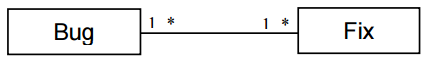
\includegraphics[scale=0.5]{media/bug-taxo-class-diag.png}
    \caption{Class diagram showing the relationship between bugs and fixed
    \label{fig:bug-taxo-diag}}
\end{figure}

\begin{figure}[h!]
  \centering
    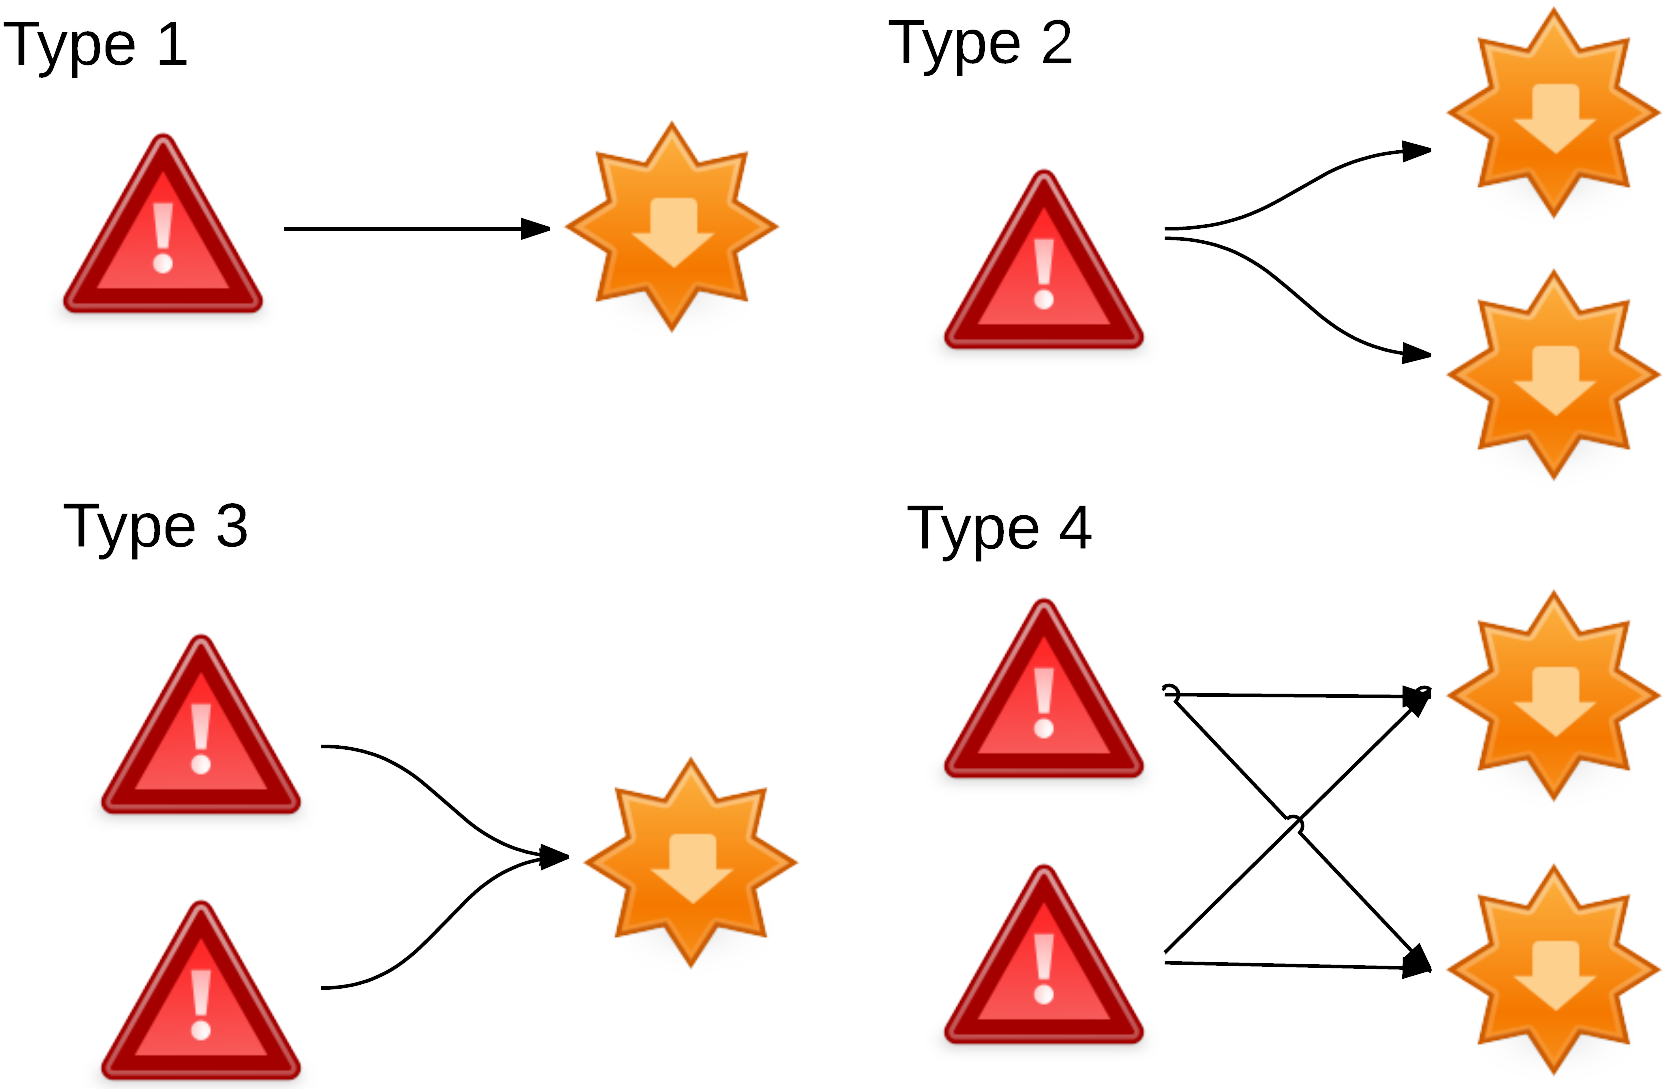
\includegraphics[scale=0.6]{media/bug-taxo.png}
    \caption{Proposed Taxonomy of Bugs
    \label{fig:bug-taxo}}
\end{figure}

The first and second types are the ones we intuitively know about. Type
1 refers to a bug being fixed in one single location (i.e., one file),
while Type 2 refers to bugs being fixed in more than one location. In
Figure 2, only two locations are shown for the sake of clarity, but many
more locations could be involved in the fix of a bug. Type 3 refers to
multiple bugs that are fixed in the exact same location. Type 4 is an
extension of Type 3, where multiple bugs are resolved by modifying the
same set of locations. Note that Type 3 and Type 4 bugs are not
duplicates, they may occur when different features of the system fail
due to the same root causes (faults). We conjecture that knowing the
proportions of each type of bugs in a system may provide insight into
the quality of the system. Knowing, for example, that in a given system
the proportion of Type 2 and 4 bugs is high may be an indication of poor
system quality since many fixes are needed to address these bugs. In
addition, the existence of a high number of Types 3 and 4 bugs calls for
techniques that can effectively find bug reports related to an incoming
bug during triaging. This is similar to the many studies that exist on
detection of duplicates (e.g., (Runeson, Alexandersson, and Nyholm 2007;
Sun et al. 2010; Nguyen et al. 2012)), except that we are not looking
for duplicates but for related bugs (bugs that are due to failures of
different features of the system, caused by the same faults). To our
knowledge, there is no study that empirically examines bug data with
these types in mind, which is the main objective of this section. More
particularly, we are interested in the following research questions:

\begin{itemize}
    \item RQ1: What are the proportions of different types of bugs?
    \item RQ2: How complex is each type of bugs?
    \item RQ3: Are bug types predictable at opening time?
\end{itemize}

\section{Study Design}\label{study-design}

The goal of this study is to analyze the location of bug fixes, with the
purpose of classifying bug fixes into types. More specifically, this
study aims to answer the following three research questions:

\begin{itemize}
\item
  \textbf{RQ\(_1\):} \emph{What are the proportions of different types
  of bugs?} This research question aims to what extent bug can be
  classified according to their fix-locations and the proportion of each
  types. Specifically, we investigate if different types of bugs exists
  at all and if the proportion of different types in non-negligible. As
  discussed earlier, knowing, for example, that bugs of Type 3 and 4 are
  the most predominant ones suggests that we need to investigate
  techniques to help detect whether an incoming bug is of Types 3 and 4
  by examining historical data. Similarly, if we can automatically
  identify a bug that is related to another one that has been fixed then
  we can reuse the results of reproducing the first bug in reproducing
  the second one.
\item
  \textbf{RQ\(_2\):} \emph{How complex is each type of bugs?} This
  second research question aims to investigate the complexity of the
  different types of bug. More specifically, we analyze and discuss the
  complexity of different types of bugs using code and process metrics
  both. For the code aspect of the complexity, we compute the number of
  different files impacted by the fix and the number of hunks and
  churns. We do not compute any statistical complexity metrics such as
  cyclomatic complexity (McCabe and Butler 1989). For the process aspect
  of complexity, we analyze the severity of the bug, the amount of
  duplicate bug report submitted, the number of times a bug report gets
  reopened, the number of comments and the time required to fix the bug.
\item
  \textbf{RQ\(_3\):} \emph{Are bug types predictable at opening time?}
  This third research questions aims at determining the predictability
  of bug types. In details, we investigate what are the best ways to
  predict the type of a bug report at submit time. Being able to build
  accurate classifiers predicting the bug type at submit time will allow
  researcher to enhance triaging approaches. Indeed, combining the
  results of our second research question with an accurate classifier
  will, for example, allow triaging approaches to assign more complex
  bug reports, based on their types, to experienced developers within
  the organization. \#\# Version control
  systems\label{sec:version-control}
\end{itemize}

Version control consists of maintaining the versions of files --- such
as source code and other software artifacts (Zeller 1997). This activity
is a complex task and cannot be performed manually on real world
project. Consequently, numerous tools have been created to help
practitioners manage the version of their software artifacts. Each
evolution of a software is a version (or revision) and each version
(revision) is linked to the one before through modifications of software
artifacts. These modifications consist of updating, adding or deleting
software artifacts. They can be referred as diff, patch or
commit\footnote{These names are not to be used interchangeably as difference exists.}.
Each diff, patch or commit have the following characteristics:

\begin{itemize}
\tightlist
\item
  Number of Files: The number of software files that have been modified,
  added or deleted.
\item
  Number of Hunks: The number of consecutive code blocks of modified,
  added or deleted lines in textual files. Hunks are used to determine,
  in each file, how many different places the developer has modified.
\item
  Number of Churns: The number of lines modified. However, the churn
  value for a line change should be at least two as the line has to be
  deleted first and then added back with the modifications.
\end{itemize}

In modern versioning systems, when maintainers make modifications to the
source code want to version it, they have to do commit. The commit
operation will version the modifications applied to one or many files.

Figure \ref{fig:branching} presents the data structure used to store a
commit. Each commit is represented as a tree. The root leaf (green)
contains the commit, tree and parent hashes as same as the author and
the description associated with the commit. The second leaf (blue)
contains the leaf hash and the hashes of the files of the project.

\begin{figure}[h!]
  \centering
    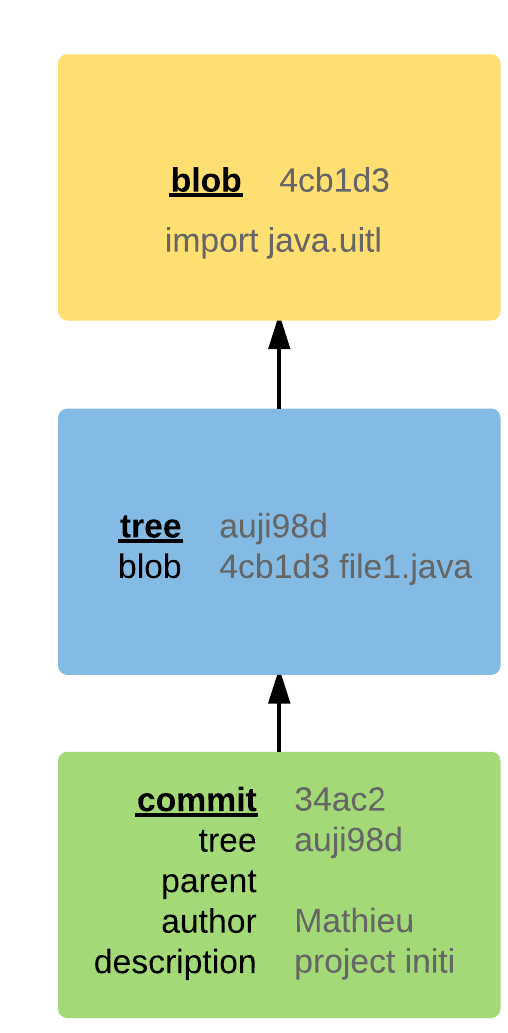
\includegraphics[scale=0.20]{media/commit-datastructure.png}
    \caption{Data structure of a commit.
    \label{fig:branching}}
\end{figure}

In this example, we can see that author ``Mathieu'' has created the file
\(file1.java\) with the message ``project init''.

\subsection{Project Tracking Systems\label{sec:issue-tracking}}

Project tracking systems allow end users to create bug reports (BRs) to
report unexpected system behavior, manager can create tasks to drive the
evolution forward and crash report (CRs) can be automatically created.
These systems are also used by development teams to keep track of the
modification induced by bug and to crash reports, and keep track of the
fixes.

\begin{figure}[h!]
    \centering
    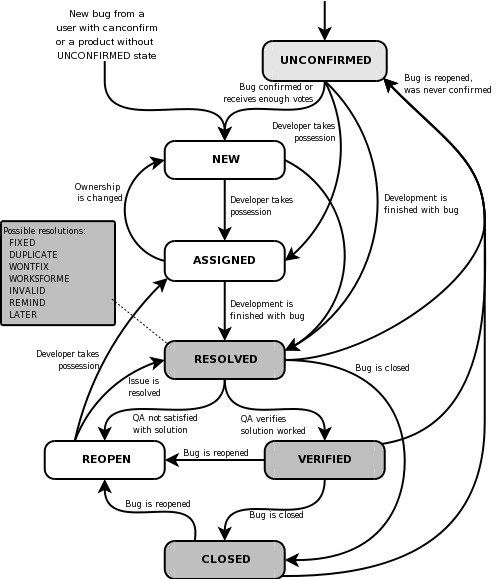
\includegraphics[scale=0.5]{media/bzLifecycle.png}
    \caption{Lifecyle of a report [@Bugzilla2008]}
    \label{fig:bug-lifecyle}
\end{figure}

Figure \ref{fig:bug-lifecyle} presents the life cycle of a report. When
a report is submitted by an end-user, it is set to the
\emph{UNCONFIRMED} state until it receives enough votes or that a user
with the proper permissions modifies its status to \emph{NEW}. The
report is then assigned to a developer to be fixed. When the report is
in the \emph{ASSIGNED} state, the assigned developer(s) starts working
on the report. A fixed report moves to the \emph{RESOLVED} state.
Developers have five different possibilities to resolve a report:
\emph{FIXED}, \emph{DUPLICATE}, \emph{WONTFIX}, \emph{WORKSFORME} and
\emph{INVALID} (Koponen 2006).

\begin{itemize}
\tightlist
\item
  RESOLVED/FIXED: A modification to the source code has been pushed,
  i.e., a changeset (also called a patch) has been committed to the
  source code management system and fixes the root problem described in
  the report.
\item
  RESOLVED/DUPLICATE: A previously submitted report is being processed.
  The report is marked as duplicate of the original report.
\item
  RESOLVED/WONTFIX: This is applied in the case where developers decide
  that a given report will not be fixed.
\item
  RESOLVED/WORKSFORME: If the root problem described in the report
  cannot be reproduced on the reported OS / hardware.
\item
  RESOLVED/INVALID: If the report is not related to the software itself.
\end{itemize}

Finally, the report is \emph{CLOSED} after it is resolved. A report can
be reopened (sent to the \emph{REOPENED} state) and then assigned again
if the initial fix was not adequate (the fix did not resolve the
problem). The elapsed time between the report marked as the new one and
the resolved status are known as the \emph{fixing time}, usually in
days. In case of task branching, the branch associated with the report
is marked as ready to be merged. Then, the person in charge (quality
assurance team, manager, ect\ldots{}) will be able to merge the branch
with the mainline. If the report is reopened: the days between the time
the report is reopened and the time it is marked again as \emph{RESOLVED
FIXED} are cumulated. Reports can be reopened many times.

Tasks follow a similar life cycle with the exception of the
\emph{UNCONFIRMED} and \emph{RESOLVED} states. Tasks are created by
management and do not need to be confirmed in order to be \emph{OPEN}
and \emph{ASSIGNED} to developers. When a task is complete, it will not
go to the \emph{RESOLVED} state, but to the \emph{IMPLEMENTED} state.
Bug and crash reports are considered as problems to eradicate in the
program. Tasks are considered as new features or amelioration to include
in the program.

Reports and tasks can have a severity (Bettenburg et al. 2008). The
severity is a classification to indicate the degree of impact on the
software. The possible severities are:

\begin{itemize}
\tightlist
\item
  blocker: blocks development and/or testing work.
\item
  critical: crashes, loss of data, severe memory leak.
\item
  major: major loss of function.
\item
  normal: regular report, some loss of functionality under specific
  circumstances.
\item
  minor: minor loss of function, or other problem where easy workaround
  is present.
\item
  trivial: cosmetic problems like misspelled words or misaligned text.
\end{itemize}

The relationship between an report or a task and the actual modification
can be hard to establish and it has been a subject of various research
studies (e.g., (Antoniol et al. 2002; Bachmann et al. 2010; Wu et al.
2011)). This reason is that they are in two different systems: the
version control system and the project tracking system. While it is
considered a good practice to link each report with the versioning
system by indicating the report \(\#id\) on the modification message,
more than half of the reports are not linked to a modification (Wu et
al. 2011).

\subsection{Context Selection}\label{context-selection}

The context of this study consists of the change history of 388 projects
belonging to two software ecosystem, namely, Apache and Netbeans. Table
\ref{table:datasets} reports, for each of them, (i) the number of
projects analyzed, (ii) size ranges in terms of the number of classes
and KLOC, (iii) the overall number of commits and issues analyzed, and
(iv) the average, minimum, and maximum length of the projects' story (in
years).

\begin{table}[h]
\begin{center}
\begin{tabular}{@{}c|c|c|c|c@{}}
\textbf{Dataset} & \textbf{R/F BR} & \textbf{CS} & \textbf{Files} & \textbf{Projects} \\ \hline \hline
Netbeans         & 53,258          & 122,632     & 30,595         & 39                \\
Apache           & 49,449          & 106,366     & 38,111         & 349               \\
Total            & 102,707         & 229,153     & 68,809         & 388               \\ \hline \hline

\end{tabular}
\end{center}

\caption{Datasets\label{table:datasets}}
\end{table}

All the analyzed projects are hosted in \emph{Git} or \emph{Mercurial}
repositories and have either a \emph{Jira} or a \emph{Bugzilla} issue
tracker associated with it. The Apache ecosystem consists in 349
projects written in various programming languages (C, C++, Java, Python,
\ldots{}) and uses \emph{Git} and \emph{Jira}. These projects represent
the Apache ecosystem in its entirety; no system has been excluded from
our study. The complete list can be found
online\footnote{https://projects.apache.org/projects.html?name}. The
Netbeans ecosystem consists in 39 projects, mostly written in Java.
Similarly to the Apache ecosystem, we did not select any of the projects
belonging to the Netbeans ecosystem but all of them. The Netbeans
community uses \emph{Bugzilla} and \emph{Mercurial}.

The choice of the ecosystems to analyze is not random, but rather driven
by the motivation to consider projects having (i) different sizes, (ii)
different architectures, and (iii) different development bases and
processes. Indeed, Apache projects are extremely various in terms of
size of the development team, purpose and technical choices (Bavota et
al. 2013). On the other side, Netbeans has a relatively stable list of
core developer and a common vision shared through the 39 related
projects (Wang, Baik, and Devanbu 2011).

Cumulatively, these datasets span from 2001 to 2014. In summary, our
consolidated dataset contains 102,707 bugs, 229,153 changesets, 68,809
files that have been modified to fix the bugs, 462,848 comments, and 388
distinct systems. We also collected 221 million lines of code modified
to fix the bugs, identified 3,284 sub-projects, and 17,984 unique
contributors to these bug report and source code version management
systems. The cumulated opening time for all the bugs reaches 10,661
working years (3,891,618 working days).

\subsection{Data Extraction and
Analysis}\label{data-extraction-and-analysis}

This subsection describes the data extraction and analysis process that
we followed to answer our research questions.

\subsubsection{What are the proportions of different types of
bugs?}\label{what-are-the-proportions-of-different-types-of-bugs}

To answer \textbf{RQ\(_1\)}, we cloned the 349 \emph{git} repositories
belonging to the Apache ecosystem and the 39 \emph{mercurial}
repositories belonging to the Netbeans ecosystem. The raw size of the
cloned source code alone, excluding binaries, images and other non-text
file, is 163 GB. Then, we extracted all the 102,707 closed issues that
have been resolved using the \emph{RESOLVED FIXED} tags. Indeed, this
study aims to classify bugs according to their fix locations. If an
issue is fixed by other means than \emph{fixing} the source code, then,
it falls outside the scope our study. In order to assign commits to
issues we used is the regular expression-based approach by Fischer et
al. (Fischer, Pinzger, and Gall, n.d.) matching the issue ID in the
commit note. Using this technique, we were able to link almost 40\%
(40,493 out of 102,707) of our resolved/fixed issues to 229,153 commits.
An issue can be fixed with several commits.

We choose not to use more complex technics like ReLink, an approach
proposed by Wu et al.(Wu et al. 2011), which considers the following
constraints: (i) matching the committer/authors with issue tracking
contributor name/email; (ii) the time interval between the commit and
the last comment posted by the same author/contributor on the issue
tracker must be less than seven days; and (iii) Vector Space Model (VSM)
cosine similarity between the commit note and the last comment referred
above or greater than 0.7 because we believe that mining more than forty
thousands issues is enough to be significant.

Using our generated consolidated dataset, we extracted the files \(f_i\)
impacted by each commit \(c_i\) for each one of our 388 projects. Then,
we classify the bugs according to the following:

\begin{itemize}
\tightlist
\item
  \textbf{Type 1:} A bug is tagged type 1 if it is fixed by modifying a
  file \(f_i\) and \(f_i\) is not involved in any other bug fix.
\item
  \textbf{Type 2:} A bug is tagged type 2 if it is fixed by modifying
  several files \(f_{i..n}\) and the files \(f_{i..n}\) are not involved
  in any other bug fix.
\item
  \textbf{Type 3:} A bug is tagged type 3 if it is fixed by modifying a
  file \(f_{i}\) and the file \(f_{i}\) is involved in fixing other
  bugs.
\item
  \textbf{Type 4:} A bug is tagged type 4 if it is fixed by modifying
  several files \(f_{i..n}\) and the files \(f_{i..n}\) are involved in
  any other bug fix.
\end{itemize}

To answer this question, we analyze whether any type is predominant in
the studied ecosystem, by testing the null hypothesis:

\begin{itemize}
\tightlist
\item
  \(H_{01}\) : The proportion of types does not change significantly
  across the studied ecosystems.
\end{itemize}

We test this hypothesis by observing both a `'global'`(across ecosystem)
and a'`local'' predominance (per ecosystem) of the different types of
bugs. We must observe these two aspects to ensure that the predominance
of a particular type of bug is not circumstantial (in few given systems
only) but is also not due to some other, unknown factors (in all systems
but not in a particular ecosystem).

We answer \textbf{RQ\(_1\)} in two steps. The first step is to use
descriptive statistics; we compute the ratio of each types to the total
number of bugs in the dataset.

In the second step, we compare the proportions of the different types of
bugs with respect to the ecosystem where the bugs were found. We build
the contingency table with these two qualitative variables (the type and
studied ecosystem) and test the null hypothesis \textbf{H\(_{01A}\)} to
assess whether the proportion of a particular type of bugs is related to
a specific ecosystem or not.

We use the Pearson's chi-squared test to reject the null hypothesis
\(H_{01A}\). Pearson's chi-squared independence test is used to analyze
the relationship between two qualitative data, in our study the type
bugs and the studied ecosystem. The results of Pearson's chi-squared
independence tests are considered statistically significant at
\(\alpha\) = 0.05. If p-value \(\le\) 0.05, we reject the null
hypothesis \(H_{01A}\) and conclude that the proportion of each types is
different for each ecosystem.

Overall, the data extraction and manipulation for \textbf{RQ\(_1\)}
(i.e., cloning repositories, linking commits to issues and tagging
issues by type) took thirteen weeks on two Linux servers having 1
quadcore 3.10 GHz CPU and 12 GB of RAM each.

\subsubsection{How complex is each type of
bugs?}\label{how-complex-is-each-type-of-bugs}

To answer \textbf{RQ\(_2\)} we went through the 40,493 resolved/fixed
issues and the linked 229,153 commits in order to compute code and
process metrics for each of them. These metrics will then be used to
assess the complexity of a bug. The computed process metrics are:

\begin{itemize}
\tightlist
\item
  The time \(t\) it took to resolve issue \(i\).
\item
  The number of issues \(dup\) tagged as duplicate of issue \(i\).
\item
  The number of time issue \(i\) got reopen \(reop\).
\item
  The number of comments \(comment\) on issue \(i\).
\item
  The severity \(sev\) of the issue \(i\).
\end{itemize}

The computed code metrics are:

\begin{itemize}
\tightlist
\item
  The number of files \(f\) impacted by issue \(i\).
\item
  The number of commit \(c\) required to fix the issue \(i\).
\item
  The number of hunks \(h\) required to fix the issue \(i\).
\item
  The number of churns \(ch\) required to fix the issue \(i\).
\end{itemize}

We address the relation between types and the complexity of the bugs in
using our metrics. We analyze whether Types 2 and 4 bugs are more
complex to handle than Types 1 and 3 bugs, by testing the null
hypotheses:

\begin{itemize}
\tightlist
\item
  \(H_{02}\): The complexity of bug types is not significantly different
  from type to type.
\end{itemize}

To test our hypothesis, we build a contingency table with the
qualitative variables and the dependent variable for each type.

We use the Pearson's chi-squared test to reject the null hypothesis
\(H_{02}\). The results of Pearson's chi-squared independence tests are
considered statistically significant at \(\alpha\) = 0.05. If a p-value
\(\le\) 0.05, we reject the null hypothesis \(H_{02}\) and conclude that
the complexity of bug is related to its type.

\subsubsection{Are bug types predictable at opening
time?}\label{are-bug-types-predictable-at-opening-time}

This third research question aims at determining the predictability of
bug types. In details, we investigate what are the best ways to predict
the type of a bug report at submit time. Being able to build accurate
classifiers predicting the bug type at submit time will allow researcher
to enhance triaging approaches. Indeed, combining the results of our
second research question with an accurate classifier will, for example,
allow triaging approaches to assign more complex bug reports, based on
their types, to experienced developers within the organization. In order
to answer this question we used the text contained on the bug report and
the text from the comment posted the first 48 hours after the report's
opening as they are likely to give some additional information about the
bug itself. Then, we removed all the stopwords (i.e.~the, or, she, he)
and truncated the remaining words to their roots (i.e.~writing becomes
write, failure becomes fail and so on). Finally, we apply the compute
tfidf on the transformed text and create three different datasets using
the n-grams technique. The datasets are 1, 2 and 3-grams. In order to
build the classifier, we use three well-known machine learning
techniques that are proven to yield satisfactory results while working
on bug reports: svm, random forest and linear regression.

We analyze whether bug types are predictable by testing the null
hypothesis:

\begin{itemize}
\tightlist
\item
  \(H_{03}\): Bug types classifiers are not accurate.
\end{itemize}

To test our hypothesis, we predict the bug type of the most complex
type, according to \textbf{RQ\(_2\)}, in ten different projects. The
results of the prediction tests are considered pertinent if they
significantly improve upon a random classifier.

\section{Analysis of the Results}\label{analysis-of-the-results}

This section reports the analysis of the results aiming at answering our
three research questions.

\subsection{What are the proportions of different types of
bugs?}\label{what-are-the-proportions-of-different-types-of-bugs-1}

\begin{table*}[]
\centering
\small
\caption{Contingency table and Pearson's chi-squared tests}
\label{tab:contingency-table}
\resizebox{\textwidth}{!}{%
\begin{tabular}{cccccc}
Ecosystem & T1                 & T2               & T3                & T4                & Pearson's chi-squared p-Value                          \\ \rowcolor{gray!25}
Apache    & 1968  (14.3 \%)   & 1248  (9.1 \%)  & 3101  (22.6 \%)  &7422  ( 54 \%)    &  \\ \rowcolor{gray!25}
Netbeans  & 776  (2.9 \%)     & 240  (0.9 \%)   & 8372  (31.3 \%)  & 17366  (64.9 \%) &  \textless0.01                               \\ \rowcolor{gray!25}
Overall   & 2744  (6.8 \%)    & 1488  (3.7 \%)  & 11473  (28.3 \%) & 24788  (61.2 \%) &                                \\
\end{tabular}
}
\end{table*}


Table \ref{tab:contingency-table} presents a contingency table and the
results of the Pearson's chi-squared tests we performed on each types of
bug. In addition to presenting bug types 1 to 4, Table
\ref{tab:contingency-table} also presents grouping of bug types: Types 1
and 2 versus Types 3 and 4.

Types 3 (22.6\% and 54\%) and 4 (31.3\% and 64.9\%) are predominant
compared to types 1 (14.3\% and 9.1\%) and 2 (6.8\% and 3.7\%) for the
Apache and the Netbeans ecosystems, respectively. Overall, the
proportion of different types of bug is as follows: 6.8\%, 3.7\%,
28.3\%, 61.2\% for types 1, 2, 3 and 4, respectively. The result of the
Pearson's test is below 0.01. As a reminder, we consider results of
Pearson's tests statistically significant at \(\alpha \textless0.05\).
Consequently, we reject to null hypothesis \(H_{01}\) and conclude that
there is a predominance of Types 3 and 4 in all different ecosystems and
this observation is not related to a specific ecosystem. When combined
into our first group, Types 1 \& 2 versus Types 3 \& 4, there are
significantly more Types 3 and 4 (89.5 \%) than Types 1 and 2 (10.5 \%).

\subsection{How complex is each type of
bugs?}\label{how-complex-is-each-type-of-bugs-1}

To answer\textbf{RQ\(_2\)}, we analyze the complexity of each bug in
terms of duplication, fixing time, comments, reopenning, files impacted,
severity, changesets, hunks and chunks.

Figure \ref{fig:boxplots} presents nine boxplots describing our
complexity metric for each type of each ecosystem. In each sub-figure,
the book plates are organized as follows: (a) Types 1 to 4 bugs for the
Apache ecosystem, (b) Types 1 to 4 bugs for the Netbeans ecosystem and
(c) Types 1 to 4 bugs for both ecosystems combined. For all the metrics,
except the severity, the median is close to zero and we can observe many
outliers. Tables \ref{tab:apache-eco}, \ref{tab:netbeans-eco} and
\ref{tab:overall-eco} present descriptive statistics about each metric
for each type for the Apache ecosystem, the Netbeans ecosystem, and both
ecosystems combined, respectively. The descriptive statistics used are
\(\mu\):mean, \(\sum\):sum, \(\hat{x}\):median, \(\sigma\):standard
deviation and \(\%\):percentage. In addition, to the descriptive
statistics, these tables present matrices of Mann-Whitney test for each
metric and type. We added the \checkmark\textasciitilde{}symbol to the
Mann-Whitney tests results columns when the value is statistically
significant (e.g. \(\alpha \textless 0.05\)) and \xmark otherwise.

Finally, Table \ref{tab:chi-rq2} presents the Pearson's chi-squared test
results for each complexity metric for Types 1 to 4 and our two types
combination. In what follows, we present our findings for each
complexity metric. Complexity metrics are divided into two groups: (a)
process and (b) code metrics. Process metrics refer to metrics that have
been extracted from the project tracking system (i.e., fixing time,
comments, reopening and severity). Code metrics are directly computed
using the source code used to fix a given bug (i.e., files impacted,
changesets required, hunks and chunks). We acknowledge that these
complexity metrics only represent an abstraction of the actual
complexity of a given bug as they cannot account for the actual thought
process and expertise required to craft a fix. However, we believe that
they are an accurate abstraction. Moreover, they are used in several
studies in the field to approximate the complexity of a bug (Weiß,
Zimmermann, and Zeller 2007; Saha, Khurshid, and Perry 2014; Nam, Pan,
and Kim 2013; Anvik, Hiew, and Murphy 2006; Nagappan and Ball 2005).

\begin{figure*}
\centering
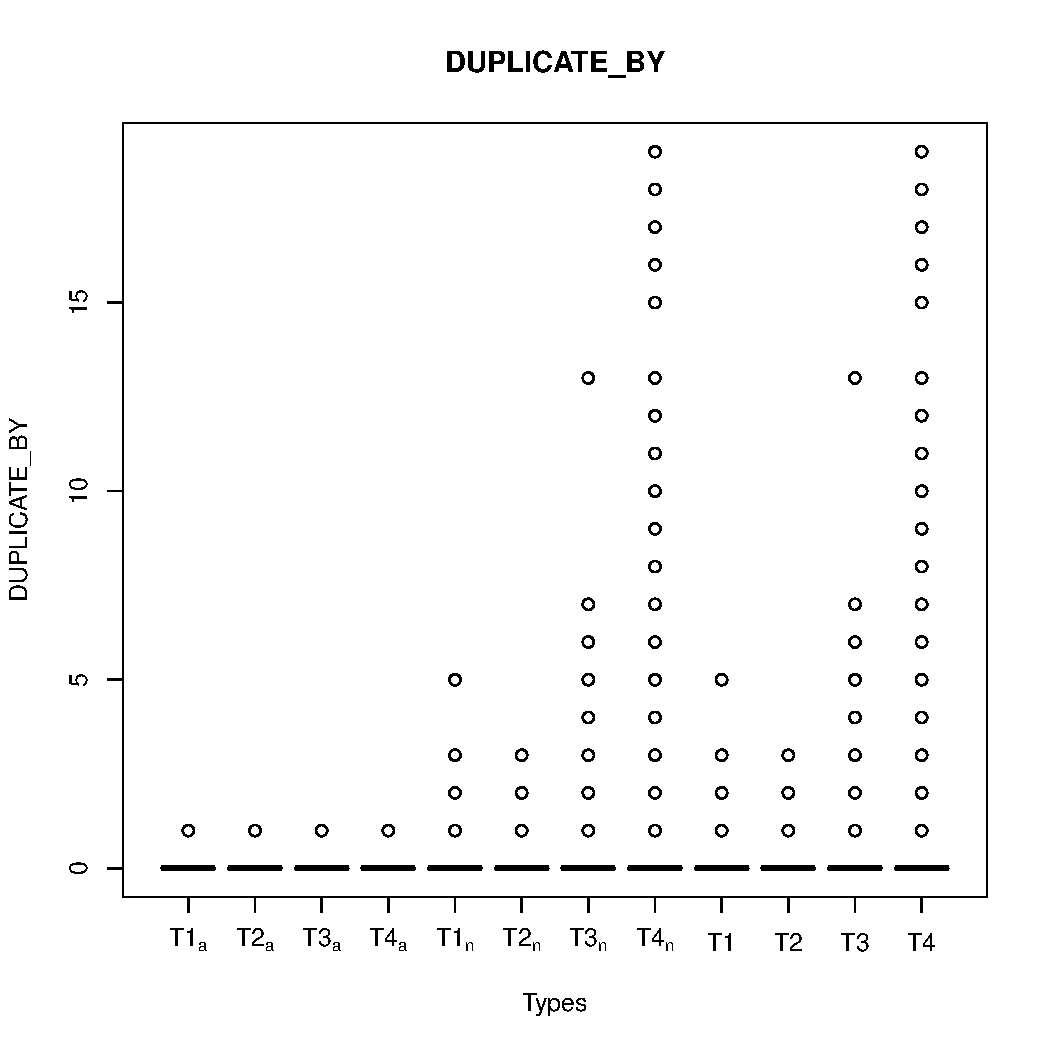
\includegraphics[page=1, width=0.45\textwidth]{extract/Rplots}
\includegraphics[page=2, width=0.45\textwidth]{extract/Rplots} \\
\includegraphics[page=3, width=0.45\textwidth]{extract/Rplots}
\includegraphics[page=4, width=0.45\textwidth]{extract/Rplots} \\
\includegraphics[page=5, width=0.45\textwidth]{extract/Rplots}
\includegraphics[page=6, width=0.45\textwidth]{extract/Rplots}
\label{fig:boxplots}
\end{figure*}

\begin{figure*}
\centering
\includegraphics[page=7, width=0.45\textwidth]{extract/Rplots}
\includegraphics[page=8, width=0.45\textwidth]{extract/Rplots} \\
\includegraphics[page=9, width=0.45\textwidth]{extract/Rplots}
\caption{Complexity metrics boxplots. From left to right and top to bottom: Duplicate, Fixing time, Comments, Reopening, Files impacted, Severity, Changesets, Hunks and Chunks.
\label{fig:boxplots}}

\end{figure*}


% Please add the following required packages to your document preamble:
% \usepackage{graphicx}
\begin{table*}[]
\centering
\small
\caption{Apache Ecosystem Complexity Metrics Comparison and Mann-whitney test results. \\ $\mu$:mean, $\sum$:sum, $\hat{x}$:median, $\sigma$:standard deviation, $\%$:percentage}
\label{tab:apache-eco}
\begin{tabular}{ccccccc|ccccc}

Types & Metric &$\mu$ & $\sum$ & $\hat{x}$ & $\sigma$ & $\%$ & T1 & T2 & T3 & T4 \\ \hline \rowcolor{gray!25}
& Dup. & 0.026 & 51 & 0 & 0.2 & 14.8 & n.a & \xmark (0.53) & \checkmark  (\textless 0.05) & \xmark (0.45)  \\ \rowcolor{gray!25}
& Tim. & 91.574 & 180217 & 4 & 262 & 21.8 & n.a & \checkmark  (\textless 0.05) & \checkmark  (\textless 0.05) & \checkmark  (\textless 0.05)  \\ \rowcolor{gray!25}
& Com. & 4.355 & 8571 & 3 & 4.7 & 9.5 & n.a & \checkmark  (\textless 0.05) & \xmark (0.17) & \checkmark  (\textless 0.05)  \\ \rowcolor{gray!25}
& Reo. & 0.062 & 122 & 0 & 0.3 & 13.8 & n.a & \xmark (0.29) & \checkmark  (\textless 0.05) & \checkmark  (\textless 0.05)  \\ \rowcolor{gray!25}
T1 & Fil. & 0.991 & 1950 & 1 & 0.1 & 3.7 & n.a & \checkmark  (\textless 0.05) & \xmark (0.28) & \checkmark  (\textless 0.05)  \\ \rowcolor{gray!25}
& Sev. & 3.423 & 6737 & 4 & 1.3 & 13.2 & n.a & \xmark (0.18) & \checkmark  (\textless 0.05) & \checkmark  (\textless 0.05)  \\ \rowcolor{gray!25}
& Cha. & 1 & 1968 & 1 & 0 & 1.9 & n.a & \checkmark  (\textless 0.05) & \checkmark  (\textless 0.05) & \checkmark  (\textless 0.05)  \\ \rowcolor{gray!25}
& Hun. & 3.814 & 7506 & 3 & 2.4 & 0 & n.a & \checkmark  (\textless 0.05) & \checkmark  (\textless 0.05) & \checkmark  (\textless 0.05)  \\ \rowcolor{gray!25}
& Chur. & 18.761 & 36921 & 7 & 48.6 & 0 & n.a & \checkmark  (\textless 0.05) & \xmark (0.09) & \checkmark  (\textless 0.05)  \\


 & Dup. & 0.022 & 28 & 0 & 0.1 & 8.1 & \xmark (0.53) & n.a & \xmark (0.16) & \xmark (0.19)  \\
 & Tim. & 115.158 & 143717 & 8 & 294.1 & 17.4 & \checkmark  (\textless 0.05) & n.a & \checkmark  (\textless 0.05) & \checkmark  (\textless 0.05)  \\
 & Com. & 5.041 & 6291 & 4 & 4.7 & 7 & \checkmark  (\textless 0.05) & n.a & \checkmark  (\textless 0.05) & \checkmark  (\textless 0.05)  \\
 & Reo. & 0.071 & 89 & 0 & 0.3 & 10.1 & \xmark (0.29) & n.a & \checkmark  (\textless 0.05) & \xmark (0.59)  \\
T2 & Fil. & 4.381 & 5468 & 2 & 20.4 & 10.5 & \checkmark  (\textless 0.05) & n.a & \checkmark  (\textless 0.05) & \checkmark  (\textless 0.05)  \\
 & Sev. & 3.498 & 4365 & 4 & 1.2 & 8.6 & \xmark (0.18) & n.a & \checkmark  (\textless 0.05) & \checkmark  (\textless 0.05)  \\
 & Cha. & 4.681 & 5842 & 2 & 20.4 & 5.5 & \checkmark  (\textless 0.05) & n.a & \checkmark  (\textless 0.05) & \checkmark  (\textless 0.05)  \\
 & Hun. & 561.995 & 701370 & 14 & 13628.2 & 3.9 & \checkmark  (\textless 0.05) & n.a & \checkmark  (\textless 0.05) & \checkmark  (\textless 0.05)  \\
 & Chur. & 14184.869 & 17702716 & 88 & 400710.2 & 8 & \checkmark  (\textless 0.05) & n.a & \checkmark  (\textless 0.05) & \checkmark  (\textless 0.05)  \\

 \rowcolor{gray!25}
 & Dup. & 0.016 & 50 & 0 & 0.1 & 14.5 & \checkmark  (\textless 0.05) & \xmark (0.16) & n.a & \checkmark  (\textless 0.05)  \\ \rowcolor{gray!25}
 & Tim. & 35.892 & 111300 & 1 & 151.8 & 13.5 & \checkmark  (\textless 0.05) & \checkmark  (\textless 0.05) & n.a & \checkmark  (\textless 0.05)  \\ \rowcolor{gray!25}
 & Com. & 4.422 & 13712 & 3 & 4.4 & 15.2 & \xmark (0.17) & \checkmark  (\textless 0.05) & n.a & \checkmark  (\textless 0.05)  \\ \rowcolor{gray!25}
 & Reo. & 0.033 & 101 & 0 & 0.2 & 11.5 & \checkmark  (\textless 0.05) & \checkmark  (\textless 0.05) & n.a & \checkmark  (\textless 0.05)  \\ \rowcolor{gray!25}
 T3 & Fil. & 0.994 & 3081 & 1 & 0.1 & 5.9 & \xmark (0.28) & \checkmark  (\textless 0.05) & n.a & \checkmark  (\textless 0.05)  \\ \rowcolor{gray!25}
 & Sev. & 3.644 & 11300 & 4 & 1.1 & 22.2 & \checkmark  (\textless 0.05) & \checkmark  (\textless 0.05) & n.a & \checkmark  (\textless 0.05)  \\ \rowcolor{gray!25}
 & Cha. & 1 & 3101 & 1 & 0 & 2.9 & \checkmark  (\textless 0.05) & \checkmark  (\textless 0.05) & n.a & \checkmark  (\textless 0.05)  \\ \rowcolor{gray!25}
 & Hun. & 4.022 & 12472 & 3 & 3.4 & 0.1 & \checkmark  (\textless 0.05) & \checkmark  (\textless 0.05) & n.a & \checkmark  (\textless 0.05)  \\ \rowcolor{gray!25}
 & Chur. & 16.954 & 52573 & 6 & 49.8 & 0 & \xmark (0.09) & \checkmark  (\textless 0.05) & n.a & \checkmark  (\textless 0.05)  \\


& Dup. & 0.029 & 216 & 0 & 0.2 & 62.6 & \xmark (0.45) & \xmark (0.19) & \checkmark  (\textless 0.05) & n.a  \\
& Tim. & 52.76 & 391586 & 4 & 182.2 & 47.4 & \checkmark  (\textless 0.05) & \checkmark  (\textless 0.05) & \checkmark  (\textless 0.05) & n.a  \\
& Com. & 8.313 & 61701 & 5 & 10.2 & 68.3 & \checkmark  (\textless 0.05) & \checkmark  (\textless 0.05) & \checkmark  (\textless 0.05) & n.a  \\
& Reo. & 0.077 & 570 & 0 & 0.3 & 64.6 & \checkmark  (\textless 0.05) & \xmark (0.59) & \checkmark  (\textless 0.05) & n.a  \\
T4 & Fil. & 5.633 & 41805 & 3 & 14 & 79.9 & \checkmark  (\textless 0.05) & \checkmark  (\textless 0.05) & \checkmark  (\textless 0.05) & n.a  \\
& Sev. & 3.835 & 28466 & 4 & 1 & 56 & \checkmark  (\textless 0.05) & \checkmark  (\textless 0.05) & \checkmark  (\textless 0.05) & n.a  \\
& Cha. & 12.861 & 95455 & 4 & 52.2 & 89.7 & \checkmark  (\textless 0.05) & \checkmark  (\textless 0.05) & \checkmark  (\textless 0.05) & n.a  \\
& Hun. & 2305.868 & 17114149 & 30 & 58094.7 & 96 & \checkmark  (\textless 0.05) & \checkmark  (\textless 0.05) & \checkmark  (\textless 0.05) & n.a  \\
& Chur. & 27249.773 & 202247816 & 204 & 320023.5 & 91.9 & \checkmark  (\textless 0.05) & \checkmark  (\textless 0.05) & \checkmark  (\textless 0.05) & n.a

\end{tabular}%
\end{table*}
 
\begin{table}[]
\centering
\small
\caption{Netbeans Ecosystem Complexity Metrics Comparison and Mann-whitney test results. \hspace{\textwidth} $\mu$:mean, $\sum$:sum, $\hat{x}$:median, $\sigma$:standard deviation, $\%$:percentage}
\label{tab:netbeans-eco}
\resizebox{\textwidth}{!}{%
\begin{tabular}{ccccccc|ccccc}

Types & Metric &$\mu$ & $\sum$ & $\hat{x}$ & $\sigma$ & $\%$ & T1 & T2 & T3 & T4 \\ \hline \rowcolor{gray!25}

& Dup. & 0.086 & 67 & 0 & 0.4 & 2.5 & n.a & \xmark (0.39) & \xmark (0.24) & \xmark (0.86) \\  \rowcolor{gray!25}
& Tim. & 92.759 & 71981 & 10 & 219.1 & 2.3 & n.a & \checkmark  (\textless 0.05) & \xmark (0.15) & \checkmark  (\textless 0.05) \\  \rowcolor{gray!25}
& Com. & 4.687 & 3637 & 3 & 4.1 & 2.4 & n.a & \checkmark  (\textless 0.05) & \xmark (0.83) & \checkmark  (\textless 0.05)  \\  \rowcolor{gray!25}
& Reo. & 0.054 & 42 & 0 & 0.3 & 1.9 & n.a & \xmark (0.1) & \xmark (0.58) & \checkmark  (\textless 0.05)  \\  \rowcolor{gray!25}
T1 & Fil. & 1.735 & 1346 & 1 & 13.2 & 0.8 & n.a & \checkmark  (\textless 0.05) & \checkmark  (\textless 0.05) & \checkmark  (\textless 0.05)  \\  \rowcolor{gray!25}
& Sev. & 4.314 & 3348 & 3 & 1.5 & 3.1 & n.a & \xmark (0.66) & \checkmark  (\textless 0.05) & \checkmark  (\textless 0.05)  \\  \rowcolor{gray!25}
& Cha. & 1.085 & 842 & 1 & 0.4 & 2 & n.a & \xmark (0.99) & \xmark (0.26) & \checkmark  (\textless 0.05)  \\  \rowcolor{gray!25}
& Hun. & 4.405 & 3418 & 3 & 7 & 0.5 & n.a & \checkmark  (\textless 0.05) & \xmark (0.13) & \checkmark  (\textless 0.05)  \\  \rowcolor{gray!25}
& Chur. & 5.089 & 3949 & 2 & 12.5 & 0.3 & n.a & \checkmark  (\textless 0.05) & \checkmark  (\textless 0.05) & \checkmark  (\textless 0.05)  \\


 & Dup. & 0.067 & 16 & 0 & 0.3 & 0.6 & \xmark (0.39) & n.a & \xmark (0.73) & \xmark (0.39) \\
 & Tim. & 111.9 & 26856 & 16 & 308.6 & 0.9 & \checkmark  (\textless 0.05) & n.a & \checkmark  (\textless 0.05) & \xmark (0.41) \\
 & Com. & 4.433 & 1064 & 3 & 4 & 0.7 & \checkmark  (\textless 0.05) & n.a & \checkmark  (\textless 0.05) & \checkmark  (\textless 0.05) \\
 & Reo. & 0.079 & 19 & 0 & 0.3 & 0.9 & \xmark (0.1) & n.a & \xmark (0.11) & \xmark (0.97) \\
T2 & Fil. & 8.804 & 2113 & 2 & 42.7 & 1.3 & \checkmark  (\textless 0.05) & n.a & \checkmark  (\textless 0.05) & \checkmark  (\textless 0.05) \\
 & Sev. & 4.362 & 1047 & 3 & 1.5 & 1 & \xmark (0.66) & n.a & \checkmark  (\textless 0.05) & \checkmark  (\textless 0.05) \\
 & Cha. & 1.075 & 258 & 1 & 0.3 & 0.6 & \xmark (0.99) & n.a & \xmark (0.5) & \checkmark  (\textless 0.05)  \\
 & Hun. & 21.887 & 5253 & 8 & 62.7 & 0.7 & \checkmark  (\textless 0.05) & n.a & \checkmark  (\textless 0.05) & \checkmark  (\textless 0.05) \\
 & Chur. & 32.263 & 7743 & 8 & 125.8 & 0.7 & \checkmark  (\textless 0.05) & n.a & \checkmark  (\textless 0.05) & \checkmark  (\textless 0.05)  \\

 \rowcolor{gray!25}
& Dup. & 0.074 & 620 & 0 & 0.4 & 23.3 & \xmark (0.24) & \xmark (0.73) & n.a & \checkmark  (\textless 0.05)  \\  \rowcolor{gray!25}
& Tim. & 87.033 & 728642 & 9 & 233.6 & 23.8 & \xmark (0.15) & \checkmark  (\textless 0.05) & n.a & \checkmark  (\textless 0.05) \\  \rowcolor{gray!25}
& Com. & 4.73 & 39599 & 3 & 4.3 & 26.5 & \xmark (0.83) & \checkmark  (\textless 0.05) & n.a & \checkmark  (\textless 0.05)  \\  \rowcolor{gray!25}
& Reo. & 0.06 & 499 & 0 & 0.3 & 22.7 & \xmark (0.58) & \xmark (0.11) & n.a & \checkmark  (\textless 0.05)  \\  \rowcolor{gray!25}
T3 & Fil. & 1.306 & 10932 & 1 & 5.1 & 6.8 & \checkmark  (\textless 0.05) & \checkmark  (\textless 0.05) & n.a & \checkmark  (\textless 0.05) \\  \rowcolor{gray!25}
& Sev. & 4.021 & 33666 & 3 & 1.4 & 31.4 & \checkmark  (\textless 0.05) & \checkmark  (\textless 0.05) & n.a & \checkmark  (\textless 0.05) \\  \rowcolor{gray!25}
& Cha. & 1.065 & 8917 & 1 & 0.3 & 21 & \xmark (0.26) & \xmark (0.5) & n.a & \checkmark  (\textless 0.05) \\  \rowcolor{gray!25}
& Hun. & 5.15 & 43115 & 3 & 12.4 & 5.8 & \xmark (0.13) & \checkmark  (\textless 0.05) & n.a & \checkmark  (\textless 0.05) \\  \rowcolor{gray!25}
& Chur. & 6.727 & 56317 & 2 & 22 & 4.9 & \checkmark  (\textless 0.05) & \checkmark  (\textless 0.05) & n.a & \checkmark  (\textless 0.05)  \\


 & Dup. & 0.113 & 1959 & 0 & 0.7 & 73.6 & \xmark (0.86) & \xmark (0.39) & \checkmark  (\textless 0.05) & n.a \\
 & Tim. & 128.833 & 2237319 & 13 & 332.8 & 73 & \checkmark  (\textless 0.05) & \xmark (0.41) & \checkmark  (\textless 0.05) & n.a \\
 & Com. & 6.058 & 105202 & 4 & 6.7 & 70.4 & \checkmark  (\textless 0.05) & \checkmark  (\textless 0.05) & \checkmark  (\textless 0.05) & n.a \\
 & Reo. & 0.094 & 1639 & 0 & 0.4 & 74.5 & \checkmark  (\textless 0.05) & \xmark (0.97) & \checkmark  (\textless 0.05) & n.a & \\
T4 & Fil. & 8.408 & 146019 & 4 & 25.1 & 91 & \checkmark  (\textless 0.05) & \checkmark  (\textless 0.05) & \checkmark  (\textless 0.05) & n.a \\
 & Sev. & 3.982 & 69159 & 3 & 1.4 & 64.5 & \checkmark  (\textless 0.05) & \checkmark  (\textless 0.05) & \checkmark  (\textless 0.05) & n.a \\
 & Cha. & 1.871 & 32494 & 2 & 1.2 & 76.4 & \checkmark  (\textless 0.05) & \checkmark  (\textless 0.05) & \checkmark  (\textless 0.05) & n.a \\
 & Hun. & 40.195 & 698022 & 13 & 98.3 & 93.1 & \checkmark  (\textless 0.05) & \checkmark  (\textless 0.05) & \checkmark  (\textless 0.05) & n.a  \\
 & Chur. & 61.893 & 1074830 & 15 & 178.6 & 94 & \checkmark  (\textless 0.05) & \checkmark  (\textless 0.05) & \checkmark  (\textless 0.05) & n.a

\end{tabular}%
}
\end{table}


\begin{table*}[]
\centering
\small
\caption{Apache and Netbeans Ecosystems Complexity Metrics Comparison and Mann-whitney test results. \hspace{\textwidth} $\mu$:mean, $\sum$:sum, $\hat{x}$:median, $\sigma$:standard deviation, $\%$:percentage}
\label{tab:overall-eco}
\resizebox{\textwidth}{!}{%
\begin{tabular}{ccccccc|ccccc}

Types & Metric &$\mu$ & $\sum$ & $\hat{x}$ & $\sigma$ & $\%$ & T1 & T2 & T3 & T4 \\ \hline \rowcolor{gray!25}
& Dup. & 0.043 & 118 & 0 & 0.3 & 3.9 & n.a & \xmark (0.09) & \xmark (0.16) & \checkmark  (\textless 0.05)  \\  \rowcolor{gray!25}
& Tim. & 91.909 & 252198 & 6 & 250.6 & 6.5 & n.a & \checkmark  (\textless 0.05) & \checkmark  (\textless 0.05) & \checkmark  (\textless 0.05)  \\  \rowcolor{gray!25}
& Com. & 4.449 & 12208 & 3 & 4.5 & 5.1 & n.a & \checkmark  (\textless 0.05) & \checkmark  (\textless 0.05) & \checkmark  (\textless 0.05)  \\  \rowcolor{gray!25}
& Reo. & 0.06 & 164 & 0 & 0.3 & 5.3 & n.a & \xmark (0.07) & \checkmark  (\textless 0.05) & \checkmark  (\textless 0.05)  \\  \rowcolor{gray!25}
T1 & Fil. & 1.201 & 3296 & 1 & 7 & 1.5 & n.a & \checkmark  (\textless 0.05) & \checkmark  (\textless 0.05) & \checkmark  (\textless 0.05)  \\  \rowcolor{gray!25}
& Sev. & 3.675 & 10085 & 4 & 1.4 & 6.4 & n.a & \xmark (0.97) & \xmark (0.17) & \checkmark  (\textless 0.05)  \\  \rowcolor{gray!25}
& Cha. & 1.024 & 2810 & 1 & 0.2 & 1.9 & n.a & \checkmark  (\textless 0.05) & \checkmark  (\textless 0.05) & \checkmark  (\textless 0.05)  \\  \rowcolor{gray!25}
& Hun. & 3.981 & 10924 & 3 & 4.3 & 0.1 & n.a & \checkmark  (\textless 0.05) & \checkmark  (\textless 0.05) & \checkmark  (\textless 0.05)  \\  \rowcolor{gray!25}
& Chur. & 14.894 & 40870 & 5 & 42.2 & 0 & n.a & \checkmark  (\textless 0.05) & \checkmark  (\textless 0.05) & \checkmark  (\textless 0.05)  \\


& Dup. & 0.03 & 44 & 0 & 0.2 & 1.5 & \xmark (0.09) & n.a & \checkmark  (\textless 0.05) & \checkmark  (\textless 0.05)  \\
& Tim. & 114.632 & 170573 & 9 & 296.4 & 4.4 & \checkmark  (\textless 0.05) & n.a & \checkmark  (\textless 0.05) & \xmark (0.15)  \\
& Com. & 4.943 & 7355 & 3 & 4.6 & 3.1 & \checkmark  (\textless 0.05) & n.a & \xmark (0.72) & \checkmark  (\textless 0.05)  \\
& Reo. & 0.073 & 108 & 0 & 0.3 & 3.5 & \xmark (0.07) & n.a & \checkmark  (\textless 0.05) & \xmark (0.47)  \\
T2 & Fil. & 5.095 & 7581 & 2 & 25.4 & 3.6 & \checkmark  (\textless 0.05) & n.a & \checkmark  (\textless 0.05) & \checkmark  (\textless 0.05)  \\
& Sev. & 3.637 & 5412 & 4 & 1.3 & 3.4 & \xmark (0.97) & n.a & \xmark (0.44) & \xmark (0.1)  \\
& Cha. & 4.099 & 6100 & 2 & 18.7 & 4.1 & \checkmark  (\textless 0.05) & n.a & \checkmark  (\textless 0.05) & \checkmark  (\textless 0.05)  \\
& Hun. & 474.881 & 706623 & 12 & 12481.7 & 3.8 & \checkmark  (\textless 0.05) & n.a & \checkmark  (\textless 0.05) & \checkmark  (\textless 0.05)  \\
& Chur. & 11902.19 & 17710459 & 62 & 366988 & 8 & \checkmark  (\textless 0.05) & n.a & \checkmark  (\textless 0.05) & \checkmark  (\textless 0.05)  \\

 \rowcolor{gray!25}
& Dup. & 0.058 & 670 & 0 & 0.4 & 22.3 & \xmark (0.16) & \checkmark  (\textless 0.05) & n.a & \checkmark  (\textless 0.05)  \\  \rowcolor{gray!25}
& Tim. & 73.21 & 839942 & 6 & 215.8 & 21.6 & \checkmark  (\textless 0.05) & \checkmark  (\textless 0.05) & n.a & \checkmark  (\textless 0.05)  \\  \rowcolor{gray!25}
& Com. & 4.647 & 53311 & 3 & 4.3 & 22.2 & \checkmark  (\textless 0.05) & \xmark (0.72) & n.a & \checkmark  (\textless 0.05)  \\  \rowcolor{gray!25}
& Reo. & 0.052 & 600 & 0 & 0.3 & 19.5 & \checkmark  (\textless 0.05) & \checkmark  (\textless 0.05) & n.a & \checkmark  (\textless 0.05)  \\  \rowcolor{gray!25}
T3 & Fil. & 1.221 & 14013 & 1 & 4.4 & 6.6 & \checkmark  (\textless 0.05) & \checkmark  (\textless 0.05) & n.a & \checkmark  (\textless 0.05)  \\  \rowcolor{gray!25}
& Sev. & 3.919 & 44966 & 3 & 1.4 & 28.4 & \xmark (0.17) & \xmark (0.44) & n.a & \checkmark  (\textless 0.05)  \\  \rowcolor{gray!25}
& Cha. & 1.048 & 12018 & 1 & 0.3 & 8.1 & \checkmark  (\textless 0.05) & \checkmark  (\textless 0.05) & n.a & \checkmark  (\textless 0.05)  \\  \rowcolor{gray!25}
& Hun. & 4.845 & 55587 & 3 & 10.7 & 0.3 & \checkmark  (\textless 0.05) & \checkmark  (\textless 0.05) & n.a & \checkmark  (\textless 0.05)  \\  \rowcolor{gray!25}
& Chur. & 9.491 & 108890 & 3 & 32.3 & 0 & \checkmark  (\textless 0.05) & \checkmark  (\textless 0.05) & n.a & \checkmark  (\textless 0.05)  \\


& Dup. & 0.088 & 2175 & 0 & 0.6 & 72.3 & \checkmark  (\textless 0.05) & \checkmark  (\textless 0.05) & \checkmark  (\textless 0.05) & n.a  \\
& Tim. & 106.056 & 2628905 & 9 & 297.9 & 67.6 & \checkmark  (\textless 0.05) & \xmark (0.15) & \checkmark  (\textless 0.05) & n.a  \\
& Com. & 6.733 & 166903 & 4 & 8 & 69.6 & \checkmark  (\textless 0.05) & \checkmark  (\textless 0.05) & \checkmark  (\textless 0.05) & n.a  \\
& Reo. & 0.089 & 2209 & 0 & 0.4 & 71.7 & \checkmark  (\textless 0.05) & \xmark (0.47) & \checkmark  (\textless 0.05) & n.a  \\
T4 & Fil. & 7.577 & 187824 & 3 & 22.4 & 88.3 & \checkmark  (\textless 0.05) & \checkmark  (\textless 0.05) & \checkmark  (\textless 0.05) & n.a  \\
& Sev. & 3.938 & 97625 & 3 & 1.3 & 61.8 & \checkmark  (\textless 0.05) & \xmark (0.1) & \checkmark  (\textless 0.05) & n.a  \\
& Cha. & 5.162 & 127949 & 2 & 29 & 85.9 & \checkmark  (\textless 0.05) & \checkmark  (\textless 0.05) & \checkmark  (\textless 0.05) & n.a  \\
& Hun. & 718.58 & 17812171 & 16 & 31804.5 & 95.8 & \checkmark  (\textless 0.05) & \checkmark  (\textless 0.05) & \checkmark  (\textless 0.05) & n.a  \\
& Chur. & 8202.463 & 203322646 & 28 & 175548.3 & 91.9 & \checkmark  (\textless 0.05) & \checkmark  (\textless 0.05) & \checkmark  (\textless 0.05) & n.a
\end{tabular}%
}
\end{table*}


\subsubsection{Duplicate}\label{duplicate}

The duplicate metric represents the number of times a bug gets resolved
using the \emph{duplicate} label while referencing one of the
\emph{resolved/fixed} bug of our dataset. The process metric is useful
to approximate the impact of a given bug on the community. For a bug to
be resolved using the \emph{duplicate}, it means that the bug has been
reported before. The more a bug gets reported by the community, the more
people are impacted enough to report it. Note that, for a bug\(\_a\) to
be resolved using the \emph{duplicate} label and referencing bug\(\_b\),
bug\(\_b\) does not have to be resolved itself. Indeed, bug\(\_b\) could
be under investigation (i.e. \emph{unconfirmed}) or being fixed (i.e.
\emph{new} or \emph{assigned}). Automatically detecting duplicate bug
report is a very active research field (Sun et al. 2011; Bettenburg,
Premraj, and Zimmermann 2008; Nguyen et al. 2012; Jalbert and Weimer
2008; Tian, Sun, and Lo 2012; Runeson, Alexandersson, and Nyholm 2007)
and a well-known measure for bug impact.

In the Apache ecosystem, the types that are most likely to get
duplicated, ordered by ascending mean duplication rate, are T3 (0.016)
\(\textless\) T2 (0.022) \(\textless\) T1 (0.026) \(\textless\) T4
(0.029) and they represent 14.8\%, 8.1\%, 14.5\% and 62.6\% of the total
duplications, respectively. The differences between duplication means by
types, however, are only significant in 33.33\% (4/12) of the case.
Indeed, the mean duplication is only significant in the following cases:
T1 vs.~T3, T3 vs.~T4. For the Apache ecosystem, we can conclude that
\(T4_{dup}^1 \gg T1_{dup}^2 \gg T3_{dup}^4\). We use the notation
\(x_{m}^r \gg y_{m}^r\) (\(x_{m}^r \ll y_{m}^r\)) to represent that
\(x\), along the metric \(m\), is significantly greater (lower) than
\(y\), along the same metric, according to the mann-whitney tests
(\(\alpha \textless 0.05\)). \(r\) represents the rank of \(x\) (\(y\))
according to \(m\) from 1 (higher percentage) to 4 (lower percentage).
In the netbeans ecosystem, we have a different order with T2 (0.067)
\textless T3 (0.074) \textless T1 (0.086) \textless T4 (0.113) and they
represent 0.6\%, 23.3\%, 2.5\% and 73.6\% of the overall duplication,
respectively. Also, we have \(T4_{dup}^1 \gg T3_{dup}^2\) for the
netbeans ecosystem.

Overall, the complexity of bug types in terms of the number of
duplicates is as follows:
\(T4_{dup}^{1} \gg T1_{dup}^{3} > T3_{dup}^{2} \gg T2_{dup}^{4}\).

\subsubsection{Fixing time}\label{fixing-time}

The fixing time metric represents the time it took for the bug report to
go from the \emph{new} state to the \emph{closed} state. If the bug
report is reopenned, then the time it took for the bug to go from the
\emph{assigned} state to the \emph{closed} state is added to the first
time. A bug report can be reopened several times and all the times are
added. In this section, the time is expressed in days {[}Weiss et al.
(2007); Zhang et al. (2012); Zhang, Gong, and Versteeg (2013)\}.

In the Apache ecosystem, the types that take the most time to fix are
\(T2_{time}^3 \gg T1_{time}^2 \gg T4_{time}^1 \gg T3_{time}^4\)

The results for the Apache ecosystem might appear surprising at first
sight. Indeed, the types requiring the fewer fix location to take longer
to fix. However, this is concordant to the finding of Saha \emph{et al.}
on long lived bugs (Saha, Khurshid, and Perry 2014) where the authors
discovered that bugs that stay open the longest are, in fact, bugs that
take the fewest locations to fix. In the Netbeans ecosystem, however,
the order of bug type along the fixing time metric is different:
\(T4_{time}^1 > T2_{time}^4 \gg T1_{time}^3 > T3_{time}^2\). This
contradicts the finding of Saha \emph{et al.}, however, they did not
study the Netbeans ecosystem in their paper (Saha, Khurshid, and Perry
2014). When combined, both ecosystem amounts in the following order
\(T2_{time}^4 > T4_{time}^1 \gg T1_{time}^3 \gg T3_{time}^2\).

\subsubsection{Comments}\label{comments}

The number of comments metric refers to the comments that have been
posted by the community on the project tracking system. This third
process metric evaluates the complexity of a given bug in a sense that
if it takes more comments (explanation) from the reporter or the
assignee to provide a fix, then the bug must be more complex to
understand. The number of comments has been shown to be useful in
assessing the complexity of bugs (Zhang, Gong, and Versteeg 2013; Zhang
et al. 2012). It is also used in bug prediction approaches (D'Ambros,
Lanza, and Robbes 2010; Bhattacharya and Neamtiu 2011).

The analysis of the Mann-Whitney test matrix, in respect of comments,
for the Apache ecosystem provides the following results:
\(T4_{comment} ^1 \gg T2_{comment}^4 \gg T3_{comment}^2 > T1_{comment}^3\).

In the Netbeans ecosystem, the bug types follows a different result:
\(T4_{comment}^1 \gg T3_{comment}^2 > T1_{comment}^3 \gg T2_{comment}^4\).

When combining both ecosystems, the results are:
\(T4_{comment}^1 \gg T2_{comment}^4 > T3_{comment}^2 \gg T1_{comment}^3\).

\subsubsection{Bug Reopening}\label{bug-reopening}

The bug reopening metric counts how many times a given bug gets
reopened.If a bug report is reopened, it means that the fix was arguably
hard to come up with or the report was hard to understand (Zimmermann et
al. 2012; Shihab et al. 2010; Lo 2013). In the Apache and Netbeans
ecosystems, we found that the order bug types of the bugs that are
reopened is the same:
\(T4_{reop}^1 > T2_{reop}^4 \gg T3_{reop}^3 \gg T1_{reop}^2\) and
\(T4_{reop}^1 > T2_{reop}^4 > T3_{reop}^2 > T1_{reop}^3\), respectively.

When combined, however, the order does change:
\(T4_{reop}^1 > T2_{reop}^4 > T1_{reop}^3 \gg T3_{reop}^2\).

\subsubsection{Severity}\label{severity}

The severity metric reports the degree of impact of the report on the
software. Predicting the severity of a given report is an active
research field (Menzies and Marcus 2008; Guo2010; Lamkanfi et al. 2010;
Tian, Lo, and Sun 2012; Valdivia Garcia and Shihab 2014; Havelund,
Holzmann, and Joshi 2015) and it helps to prioritization of fixes (Xuan
et al. 2012). The severity is a textual value (blocker, critical, major,
normal, minor, trivial) and the Mann-Whitney test only accepts numerical
input. Consequently, we had to assign numerical values to each severity.
We chose to assign values from 1 to 6 for trivial, minor, normal, major,
critical and blocker severities, respectively. The bug type ordering
according to the severity metrics is:
\(T4_{sev}^1 \gg T3_{sev}^2 \gg T2_{sev}^4 > T1_{sev}^3\),
\(T2_{sev}^4 > T1_{sev}^3 \gg T3_{sev}^2 \gg T4_{sev}^1\) and
\(T4_{sev}^1 \gg T3_{sev}^2 > T1_{sev}^3 > T2_{sev}^4\) for Apache,
Netbeans, and both combined, respectively.

\subsubsection{Files impacted}\label{files-impacted}

The number of files impacted measures how many files have been modified
for the bug report to be closed. Unsurprisingly, Types 4 and 2 are the
ones with the most files impacted. Indeed, according to their
definitions, presented in Figure \ref{fig:bug-taxo}, Types 1 and 3 only
need a modification in one location. This metric is therefore applicable
to bug Types 2 and 4 only. In Apache, type 4 structures are wider than
type 2
(\(T4_{files}^1 \gg T2_{files}^2 \gg T3_{files}^3 < = > T1_{files}^4\))
while in Netbeans, type 2 are wider
(\(T2_{files}^3 \gg T4_{files}^1 \gg T3_{files}^2 < = > T1_{files}^4\)).

Overall, types 4 impacts more files than types 2 while types 1 and 2
impacts only 1 file
(\(T4_{files}^1 \gg T2_{files}^3 \gg T3_{files}^2 < = > T1_{files}^4\)).

\subsubsection{Changesets}\label{changesets}

The changeset metrics registers how many changesets (or
commits/patch/fix) have been required to close the bug report. In the
project tracking system, changesets to resolve the bug are proposed and
analysed by the community, automated quality insurance tools and the
quality insurance team itself. Each changeset can be either accepted and
applied to the source code or dismissed. The number of changesets (or
versions of a given changeset) it takes before an integration can hint
us about the complexity of the fix. In case the bug report gets reopen
and new changesets proposed, the new changesets (after the reopening)
are added to the old ones (before the reopening). For the Apache
ecosystem, we found the following:
\(T4_{changesets}^1 \gg T2_{changesets}^2 \gg T1_{changesets}^4 <=> T3_{changesets}^3\).

In the Netbeans ecosystem, the order stays the same at the exception of
Types 1 and 2 that switch position from 3 to 2 and 2 to 3, respectively
(\(T4_{changesets}^1 \gg T1_{changesets}^3 > T2_{changesets}^4 > T3_{changesets}^2\)).

Overall, Type 4 bugs are the most complex bugs in terms of the number of
submitted changesets
(\(T4_{changesets}^1 \gg T2_{changesets}^3 \gg T3_{changesets}^2 \gg T1_{changesets}^4\)).

While results have been published on the bug-fix patterns (Pan, Kim, and
Whitehead 2008), smell introduction (Tufano et al. 2015; Eyolfson, Tan,
and Lam 2011), to the best of our knowledge, no one interested
themselves in how many iterations of a patch were required to close a
bug report beside us.

\subsubsection{Hunks}\label{hunks}

The hunks metric counts the number of consecutive code blocks of
modified, added or deleted lines in textual files. Hunks are used to
determine, in each file, how many different places a developer has
modified. This metric is widely used for bug insertion prediction (Kim
et al. 2006; Jung, Oh, and Yi 2009; Rosen, Grawi, and Shihab 2015) and
bug-fix comprehension (Pan, Kim, and Whitehead 2008). In our ecosystems,
there is a relationship between the number of files modified and the
hunks. The number of code blocks modified is likely to rise as to the
number of modified files as the hunks metric will be at least 1 per
file. We found that Types 2 and 4 bugs, that requires many files to get
fixed, are the ones that have significantly higher scores for the hunks
metric; Apache ecosystem:
\(T4_{hunks}^1 \gg T2_{hunks}^2 \gg T3_{hunks}^3 \gg T1_{hunks}^4\),
Netbeans ecosystem:
\(T4_{hunks}^1 \gg T2_{hunks}^3 \gg T3_{hunks}^2 \gg T1_{hunks}^4\), and
overall
\(T4_{hunks}^1 \gg T2_{hunks}^2 \gg T1_{hunks}^4 \gg T3_{hunks}^3\).

\subsubsection{Churns}\label{churns}

The last metrics, churns, counts the number of lines modified. The churn
value for a line change should be at least two as the line has to be
deleted first and then added back with the modifications. Once again,
this is a widely used metric in the field (Kim et al. 2006; Pan, Kim,
and Whitehead 2008; Jung, Oh, and Yi 2009; Rosen, Grawi, and Shihab
2015). Once again, Types 4 and 2 are the ones with the most churns;
Apache ecosystem
\(T4_{churns}^1 \gg T2_{churns}^2 \gg T1_{churns}^4 > T3_{churns}^3\),
Netbeans ecosystem:
\(T4_{churns}^1 \gg T2_{churns}^3 \gg T3_{churns}^2 \gg T1_{churns}^4\)
and overall :
\(T4_{churns}^1 \gg T2_{churns}^2 \gg T1_{churns}^4 \gg T3_{churns}^3\).


\begin{table}[]
\centering
\small
\caption{Pearson's chi-squared tests for complexity metrics}
\label{tab:chi-rq2}
\begin{tabular}{cccc}
Eco. & Metric & T1 vs. T2 vs.   & T1T2 v.  \\
          &     &  T3 vs. T4 & T3T4  \\ \hline \rowcolor{gray!25}
          & Dup.   & \textless0.01         & \textless0.01         \\  \rowcolor{gray!25}
          & Tim.   & \textless0.01         & \textless0.01         \\  \rowcolor{gray!25}
          & Com.   & \textless0.01         & \textless0.01         \\  \rowcolor{gray!25}
          & Reo.   & \textless0.01         & \textless0.01         \\  \rowcolor{gray!25}
Apache    & Fil.   & \textless0.01         & \textless0.01         \\  \rowcolor{gray!25}
          & Sev.   & \textless0.01         & \textless0.01         \\  \rowcolor{gray!25}
          & Cha.   & \textless0.01         & \textless0.01         \\  \rowcolor{gray!25}
          & Hun.   & \textless0.01         & \textless0.01         \\  \rowcolor{gray!25}
          & Chur.  & \textless0.01         & \textless0.01         \\
          & Dup.   & \textless0.01         & \textless0.01         \\
          & Tim.   & \textless0.01         & \textless0.01         \\
          & Com.   & \textless0.01         & \textless0.01         \\
          & Reo.   & \textless0.01         & \textless0.01         \\
Netbeans  & Fil.   & \textless0.01         & \textless0.01         \\
          & Sev.   & \textless0.01         & \textless0.01         \\
          & Cha.   & \textless0.01         & \textless0.01         \\
          & Hun.   & \textless0.01         & \textless0.01         \\
          & Chur.  & \textless0.01         & \textless0.01         \\  \rowcolor{gray!25}
          & Dup.   & \textless0.01         & \textless0.01         \\  \rowcolor{gray!25}
          & Tim.   & \textless0.01         & \textless0.01         \\  \rowcolor{gray!25}
          & Com.   & \textless0.01         & \textless0.01         \\  \rowcolor{gray!25}
          & Reo.   & \textless0.01         & \textless0.01         \\  \rowcolor{gray!25}
Overall   & Fil.   & \textless0.01         & \textless0.01         \\  \rowcolor{gray!25}
          & Sev.   & \textless0.01         & \textless0.01         \\  \rowcolor{gray!25}
          & Cha.   & \textless0.01         & \textless0.01         \\  \rowcolor{gray!25}
          & Hun.   & \textless0.01         & \textless0.01         \\  \rowcolor{gray!25}
          & Chur.  & \textless0.01         & \textless0.01
\end{tabular}
\end{table}
 
% Please add the following required packages to your document preamble:
% \usepackage{multirow}
% \usepackage{graphicx}

\definecolor{Gray}{gray}{0.85}
\begin{table*}[]
\small
\centering
\caption{Types 1\& 2 versus Types 3 \& 4 Complexity Metrics Comparison and Mann-whitney test results. \\ $\mu$:mean, $\sum$:sum, $\hat{x}$:median, $\sigma$:standard deviation, $\%$:percentage}
\label{tab:combined-one}
\resizebox{\textwidth}{!}{%
\begin{tabular}{ccccccc|cccccc}
\multirow{2}{*}{Ecosystem}
& \multirow{2}{*}{Metric}
& \multicolumn{5}{c}{Types 1 and 2}
& \multicolumn{5}{c}{Types 3 and 4} & \multirow{2}{*}{\begin{tabular}[c]{@{}c@{}}Mann-Whitney\\ p-value\end{tabular}} \\ \cline{3-12}
 &  & $\mu$ & $\sum$ & $\hat{x}$ & $\sigma$ & $\%$ & $\mu$ & $\sum$ & $\hat{x}$ & $\sigma$ & $\%$ &  &  \hline
\rowcolor{gray!25}
 & Dup & 0.025 & 79 & 0 & 0.2 & 22.9 & 0.025 & 266 & 0 & 0.2 & 77.1 & \xmark ( 0.82 )  \\ \rowcolor{gray!25}
 & Time & 100.726 & 323934 & 6 & 275.1 & 39.2 & 47.789 & 502886 & 3 & 17
 3.9 & 60.8 & \checkmark (\textless 0.05)  \\ \rowcolor{gray!25}
 & Com & 4.621 & 14862 & 3 & 4.7 & 16.5 & 7.166 & 75413 & 4 & 9.1 & 83.5 & \checkmark (\textless 0.05)  \\ \rowcolor{gray!25}
 & Reop & 0.066 & 211 & 0 & 0.3 & 23.9 & 0.064 & 671 & 0 & 0.3 & 76.1 & \xmark ( 0.74 )  \\ \rowcolor{gray!25}
 Apache & Files & 2.307 & 7418 & 1 & 12.8 & 14.2 & 4.266 & 44886 & 2 & 11.9 & 85.8 & \checkmark (\textless 0.05)  \\ \rowcolor{gray!25}
 & Severity & 3.452 & 11102 & 4 & 1.2 & 21.8 & 3.779 & 39766 & 4 & 1 & 78.2 & \checkmark (\textless 0.05)  \\ \rowcolor{gray!25}
 & Change & 2.428 & 7810 & 1 & 12.8 & 7.3 & 9.366 & 98556 & 3 & 44.2 & 92.7 & \checkmark (\textless 0.05)  \\ \rowcolor{gray!25}
 & Hunks & 220.422 & 708876 & 4 & 8491.9 & 4 & 1627.542 & 17126621 & 15 & 48799.9 & 96 & \checkmark (\textless 0.05)  \\ \rowcolor{gray!25}
 & Churns & 5516.056 & 17739637 & 15 & 249654.4 & 8.1 & 19224.593 & 202300389 & 72 & 269046.2 & 91.9 & \checkmark (\textless 0.05)  \\
& Dup & 0.082 & 83 & 0 & 0.4 & 3.1 & 0.1 & 2579 & 0 & 0.6 & 96.9 & \xmark ( 0.92 )  \\
 & Time & 97.281 & 98837 & 11 & 243.2 & 3.2 & 115.237 & 2965961 & 12 & 304.8 & 96.8 & \xmark ( 0.76 )  \\
 & Com & 4.627 & 4701 & 3 & 4 & 3.1 & 5.626 & 144801 & 4 & 6.1 & 96.9 & \checkmark (\textless 0.05)  \\
 & Reop & 0.06 & 61 & 0 & 0.3 & 2.8 & 0.083 & 2138 & 0 & 0.4 & 97.2 & \xmark ( 0.08 )  \\
Netbeans & Files & 3.405 & 3459 & 1 & 23.9 & 2.2 & 6.098 & 156951 & 2 & 21.1 & 97.8 & \checkmark (\textless 0.05)  \\
 & Severity & 4.326 & 4395 & 3 & 1.5 & 4.1 & 3.995 & 102825 & 3 & 1.4 & 95.9 & \checkmark (\textless 0.05)  \\
 & Change & 1.083 & 1100 & 1 & 0.4 & 2.6 & 1.609 & 41411 & 1 & 1.1 & 97.4 & \checkmark (\textless 0.05)  \\
 & Hunks & 8.534 & 8671 & 3 & 31.9 & 1.2 & 28.795 & 741137 & 8 & 82.7 & 98.8 & \checkmark (\textless 0.05)  \\
 & Churns & 11.508 & 11692 & 3 & 63.1 & 1 & 43.949 & 1131147 & 8 & 149.5 & 99 & \checkmark (\textless 0.05)  \\
 \rowcolor{gray!25}
 & Dup & 0.038 & 162 & 0 & 0.2 & 5.4 & 0.078 & 2845 & 0 & 0.5 & 94.6 & \checkmark (\textless 0.05)  \\
 \rowcolor{gray!25}
 & Time & 99.899 & 422771 & 7 & 267.8 & 10.9 & 95.663 & 3468847 & 8 & 275 & 89.1 & \checkmark (\textless 0.05)  \\
 \rowcolor{gray!25}
 & Com & 4.623 & 19563 & 3 & 4.6 & 8.2 & 6.073 & 220214 & 4 & 7.1 & 91.8 & \checkmark (\textless 0.05)  \\
 \rowcolor{gray!25}
 & Reop & 0.064 & 272 & 0 & 0.3 & 8.8 & 0.077 & 2809 & 0 & 0.3 & 91.2 & \xmark ( 0.21 )  \\
 \rowcolor{gray!25}
 Overall & Files & 2.57 & 10877 & 1 & 16.2 & 5.1 & 5.566 & 201837 & 2 & 18.9 & 94.9 & \checkmark (\textless 0.05)  \\
 \rowcolor{gray!25}
 & Severity & 3.662 & 15497 & 4 & 1.4 & 9.8 & 3.932 & 142591 & 3 & 1.3 & 90.2 & \checkmark (\textless 0.05)  \\
 \rowcolor{gray!25}
 & Change & 2.105 & 8910 & 1 & 11.2 & 6 & 3.86 & 139967 & 2 & 24.1 & 94 & \checkmark (\textless 0.05)  \\
 \rowcolor{gray!25}
 & Hunks & 169.553 & 717547 & 4 & 7403 & 3.9 & 492.754 & 17867758 & 9 & 26297.9 & 96.1 & \checkmark (\textless 0.05)  \\
 \rowcolor{gray!25}
 & Churns & 4194.548 & 17751329 & 10 & 217637.4 & 8 & 5610.202 & 203431536 & 13 & 145192.5 & 92 & \checkmark (\textless 0.05)  \\
\end{tabular}%
}
\end{table*}


Assuming that the complexity metrics are equal in terms of assessing the
complexity of a given bug, we scored each type with a simple system. We
counted how many times each bug type obtained each position in our nine
rankings and multiply them by 4 for the first place, 3 for the second, 2
for the third and 1 for the fourth place. We did the same simple
analysis of the rank of each type for each metric, to take into account
the frequency of bug types in our calculation, and multiply both values.
The complexity scores we calculated are as follows: 1330, 1750, 2580 and
7120 for bug types 1, 2, 3 and 4, respectively. According to these
complexity scores, types 3 and 4 are more complex than types 1 and 2. In
order to confirm or infirm the validity of our complexity scores, we ran
our experiments again. This time, we combined types 1 \& 2 and types 3
\& 4 for the two ecosystems. As shown by Table \ref{tab:combined-one},
our complexity scores are meaningful. Indeed, Types 3 \& 4 are
statistically more complex (\(\gg\)) than Types 1 \& 2 according to the
duplicate, fixing time, comments, files impacted, changesets, hunks and
churns complexity metrics. Also, Types 3 \& 4 get reopen more than types
1 \& 2, in average, but the result of the mann-whitney test is not
conclusive (i.e. \(\alpha>0.05\)). Out of our nine complexity metrics,
the only one where Types 1 \& 2 perform \emph{worst} than Types 3 \& 4
is the severity.

Consequently, we reject to null hypothesis \(H_{02}\) and conclude that
the complexity of bug is related to its type. Moreover, Types 3 and 4
bugs are more complex than Types 1 and 2 bugs across the ecosystems we
studied.

\subsection{Are bug types predictable at opening
time?}\label{are-bug-types-predictable-at-opening-time-1}

To answer \textbf{RQ\(_3\)}, we analyze the accuracy of predictors
aiming at determining the type of a bug at submit time (i.e.~when the
bug report is opened). Tables \ref{tab:1gram}, \ref{tab:2gram} and
\ref{tab:3gram} presents the results obtained while building classifiers
for the most complex type of bug. According to \textbf{RQ\(_2\)}, the
most complex type of bug, in terms of duplicate, time to fix, comments,
reopening, files changed, severity, changesets, churns and hunks, is
type 4.

In order to test our null hypothesis \(H_{03}\) (Bug types classifiers
are not accurate) we built nine different classifiers using three
different machine learning techniques: Linear regression, support vector
machines and random forest for ten different projects (5 from each
ecosystem). We selected the top 5 projects of each ecosystem with regard
to their bug report count (Ambari, Cassandra, Flume, HBase and Hive for
Apache; Cnd, Editor, Java, JavaEE and Plateform for Netbeans). For each
machine learning techniques, we built classifiers using the text
contained on the bug report and the comment of the first 48 hours as
they are likely to provide additional insights on the bug itself. We
eliminate the stop-words of the text and trim the words to their
semantical roots using wordnet. On the remaining words we compute the
tf/idf metric for groups of 1, 2 and 3 grams. The tf/idf metric is then
fed to the different machine learning techniques in order to build a
classifier. The data is separated into two parts with a 60\%-40\% ratio.
The 60\% part is used for training purposes while the 40\% is used for
testing purposes. During the training process we use the ten-folds
iteratively and, for each iteration, we change the parameters used by
the classifier building process (cost, mtry, etc). At the end of the
iterations, we select the best classifier and exercise it against the
second part of 40\%. The results we report in this section are the
performances of the nine classifier trained on 60\% of the data and
classifying the remaining 40\%. The performances of each classifier is
examined in terms of true positive, true negative, false negative and
false positive classifications. True positives and negative numbers
refer to the cases where the classifier correctly classify a report. The
false negative represents the number of reports that are classified as
non-type 4 while they are and false positive represents the number of
reports classified as type 4 while they are not. These numbers allow us
to derive three common metrics: precision, recall and f\_1 measure.

\begin{equation}
precision = \frac{TP+FN \cap TP+FP}{TP+FP}
\end{equation}

\begin{equation}
recall = \frac{TP+FN \cap TP+FP}{TP+FN}
\end{equation}

\begin{equation}
f_1 = \frac{2TP}{2TP + FP + FN}
\end{equation}

Finally, the performances of each classifier are compared to tenth
classifier. This last classifier is random classifier that will randomly
predict the type of a bug. As we are in a two-classes system (type 4 and
non-type 4), 50\% of the reports are classified as type 4 by the random
classifier. The performances of the random classifier itself are
presented in table \ref{tab:random}.

% Please add the following required packages to your document preamble:
% \usepackage{graphicx}
\begin{table}[]
\centering
\caption{Support Vector Machine, Linear Regression and Random Forest based classifiers performances while using 1 gram. \hspace{\textwidth} TP: True positive, TN: True Negative, FN: False Negative, FP: False Positive }
\label{tab:1gram}
\resizebox{\textwidth}{!}{%
\begin{tabular}{llllllllll}
\hline
Project & Reports & T4 Reports & TP & TN & FN & FP & Precision & Recall & F1 \\ \hline
\multicolumn{10}{c}{Support Vector Machine} \\ \hline
Ambari & 829 & 540 & 539 & 4 & 1 & 285 & 65.41\% & 99.81\% & 79.03\% \\
Cassandra & 340 & 199 & 193 & 5 & 6 & 136 & 58.66\% & 96.98\% & 73.11\% \\
Flume & 133 & 80 & 79 & 9 & 1 & 44 & 64.23\% & 98.75\% & 77.83\% \\
HBase & 357 & 215 & 213 & 4 & 2 & 138 & 60.68\% & 99.07\% & 75.27\% \\
Hive & 272 & 191 & 191 & 0 & 0 & 81 & 70.22\% & 100.00\% & 82.51\% \\
Cnd & 1105 & 805 & 753 & 25 & 52 & 275 & 73.25\% & 93.54\% & 82.16\% \\
Editor & 666 & 478 & 455 & 16 & 23 & 172 & 72.57\% & 95.19\% & 82.35\% \\
Java & 1090 & 693 & 676 & 37 & 17 & 360 & 65.25\% & 97.55\% & 78.20\% \\
JavaEE & 585 & 287 & 258 & 52 & 29 & 246 & 51.19\% & 89.90\% & 65.23\% \\
Platform & 969 & 573 & 467 & 110 & 106 & 286 & 62.02\% & 81.50\% & 70.44\% \\
Total & 6346 & 4061 & 3824 & 262 & 237 & 2023 & 65.40\% & 94.16\% & 77.19\% \\ \hline
\multicolumn{10}{c}{Linear Regression} \\ \hline
Ambari & 829 & 540 & 514 & 14 & 26 & 275 & 65.15\% & 95.19\% & 77.35\% \\
Cassandra & 340 & 199 & 194 & 5 & 5 & 136 & 58.79\% & 97.49\% & 73.35\% \\
Flume & 133 & 80 & 60 & 17 & 20 & 36 & 62.50\% & 75.00\% & 68.18\% \\
HBase & 357 & 215 & 212 & 5 & 3 & 137 & 60.74\% & 98.60\% & 75.18\% \\
Hive & 272 & 191 & 103 & 40 & 88 & 41 & 71.53\% & 53.93\% & 61.49\% \\
Cnd & 1105 & 805 & 762 & 26 & 43 & 274 & 73.55\% & 94.66\% & 82.78\% \\
Editor & 666 & 478 & 459 & 16 & 19 & 172 & 72.74\% & 96.03\% & 82.78\% \\
Java & 1090 & 693 & 683 & 13 & 10 & 384 & 64.01\% & 98.56\% & 77.61\% \\
JavaEE & 575 & 287 & 271 & 30 & 16 & 258 & 51.23\% & 94.43\% & 66.42\% \\
Platform & 969 & 573 & 486 & 102 & 87 & 294 & 62.31\% & 84.82\% & 71.84\% \\
Total & 6336 & 4061 & 3744 & 268 & 317 & 2007 & 65.10\% & 92.19\% & 76.31\% \\ \hline
\multicolumn{10}{c}{Random Forest} \\ \hline
Ambari & 829 & 540 & 514 & 13 & 26 & 276 & 65.06\% & 95.19\% & 77.29\% \\
Cassandra & 337 & 199 & 191 & 12 & 8 & 126 & 60.25\% & 95.98\% & 74.03\% \\
Flume & 133 & 80 & 76 & 8 & 4 & 45 & 62.81\% & 95.00\% & 75.62\% \\
HBase & 357 & 215 & 212 & 9 & 3 & 133 & 61.45\% & 98.60\% & 75.71\% \\
Hive & 272 & 191 & 190 & 3 & 1 & 78 & 70.90\% & 99.48\% & 82.79\% \\
Cnd & 1105 & 805 & 803 & 4 & 2 & 296 & 73.07\% & 99.75\% & 84.35\% \\
Editor & 666 & 478 & 476 & 3 & 2 & 185 & 72.01\% & 99.58\% & 83.58\% \\
Java & 1090 & 693 & 682 & 26 & 11 & 371 & 64.77\% & 98.41\% & 78.12\% \\
JavaEE & 575 & 287 & 252 & 59 & 35 & 229 & 52.39\% & 87.80\% & 65.63\% \\
Platform & 969 & 573 & 437 & 154 & 136 & 242 & 64.36\% & 76.27\% & 69.81\% \\
Total & 6333 & 4061 & 3833 & 291 & 228 & 1981 & 65.93\% & 94.39\% & 77.63\% \\ \hline
\end{tabular}%
}
\end{table}

For the first three classifiers (svm, linear regression and random
forest with 1-gram grouping of stemmed words) the best classifier the
random forest one with 77.63\% F\_1 measure. It is followed by SVM
(77.19\%) and, finally, linear regression (76.31\%). Regardless of the
technique used to classify the report, there is no significant
difference between ecosystems. Indeed, the p-values obtained with
chi-square tests are above 0.05. A p-value below 0.05 is a marker of
statistical significance. While random forest emerges as the most
accurate classifier, the difference between the three classifier is not
significant (p-value = 0.99).

% Please add the following required packages to your document preamble:
% \usepackage{graphicx}
\begin{table}[]
\centering
\caption{Support Vector Machine, Linear Regression and Random Forest based classifiers performances while using 2 grams. \hspace{\textwidth} TP: True positive, TN: True Negative, FN: False Negative, FP: False Positive }
\label{tab:2gram}
\resizebox{\textwidth}{!}{%
\begin{tabular}{llllllllll}
\hline
Project & Reports & T4 Reports & TP & TN & FN & FP & Precision & Recall & F1 \\ \hline
\multicolumn{10}{c}{Support Vector Machine} \\ \hline
Ambari & 829 & 540 & 525 & 12 & 15 & 277 & 65.46\% & 97.22\% & 78.24\% \\
Cassandra & 323 & 199 & 189 & 11 & 10 & 113 & 62.58\% & 94.97\% & 75.45\% \\
Flume & 133 & 80 & 74 & 15 & 6 & 38 & 66.07\% & 92.50\% & 77.08\% \\
HBase & 357 & 215 & 205 & 23 & 10 & 119 & 63.27\% & 95.35\% & 76.07\% \\
Hive & 272 & 191 & 171 & 15 & 20 & 66 & 72.15\% & 89.53\% & 79.91\% \\
Cnd & 1105 & 805 & 731 & 34 & 74 & 266 & 73.32\% & 90.81\% & 81.13\% \\
Editor & 666 & 478 & 455 & 30 & 23 & 158 & 74.23\% & 95.19\% & 83.41\% \\
Java & 1090 & 693 & 664 & 58 & 29 & 339 & 66.20\% & 95.82\% & 78.30\% \\
JavaEE & 575 & 287 & 238 & 69 & 49 & 219 & 52.08\% & 82.93\% & 63.98\% \\
Platform & 969 & 573 & 461 & 110 & 112 & 286 & 61.71\% & 80.45\% & 69.85\% \\
Total & 6319 & 4061 & 3713 & 377 & 348 & 1881 & 66.37\% & 91.43\% & 76.91\% \\ \hline
\multicolumn{10}{c}{Linear Regression} \\ \hline
Ambari & 829 & 540 & 510 & 19 & 30 & 270 & 65.38\% & 94.44\% & 77.27\% \\
Cassandra & 340 & 199 & 140 & 55 & 59 & 86 & 61.95\% & 70.35\% & 65.88\% \\
Flume & 142 & 89 & 59 & 23 & 30 & 30 & 66.29\% & 66.29\% & 66.29\% \\
HBase & 357 & 215 & 90 & 100 & 125 & 42 & 68.18\% & 41.86\% & 51.87\% \\
Hive & 272 & 191 & 176 & 8 & 15 & 73 & 70.68\% & 92.15\% & 80.00\% \\
Cnd & 1105 & 805 & 745 & 26 & 60 & 274 & 73.11\% & 92.55\% & 81.69\% \\
Editor & 666 & 478 & 453 & 27 & 25 & 161 & 73.78\% & 94.77\% & 82.97\% \\
Java & 1090 & 693 & 606 & 106 & 87 & 291 & 67.56\% & 87.45\% & 76.23\% \\
JavaEE & 575 & 287 & 245 & 70 & 42 & 218 & 52.92\% & 85.37\% & 65.33\% \\
Platform & 815 & 573 & 449 & 121 & 124 & 121 & 78.77\% & 78.36\% & 78.57\% \\
Total & 6191 & 4070 & 3473 & 555 & 597 & 1566 & 68.92\% & 85.33\% & 76.25\% \\ \hline
\multicolumn{10}{c}{Random Forest} \\ \hline
Ambari & 829 & 540 & 511 & 20 & 29 & 269 & 65.51\% & 94.63\% & 77.42\% \\
Cassandra & 340 & 199 & 176 & 22 & 23 & 119 & 59.66\% & 88.44\% & 71.26\% \\
Flume & 133 & 80 & 72 & 21 & 8 & 32 & 69.23\% & 90.00\% & 78.26\% \\
HBase & 351 & 215 & 208 & 12 & 7 & 124 & 62.65\% & 96.74\% & 76.05\% \\
Hive & 272 & 191 & 190 & 0 & 1 & 81 & 70.11\% & 99.48\% & 82.25\% \\
Cnd & 1105 & 805 & 794 & 9 & 11 & 291 & 73.18\% & 98.63\% & 84.02\% \\
Editor & 666 & 478 & 471 & 6 & 7 & 182 & 72.13\% & 98.54\% & 83.29\% \\
Java & 1099 & 702 & 673 & 43 & 29 & 354 & 65.53\% & 95.87\% & 77.85\% \\
JavaEE & 575 & 287 & 238 & 86 & 49 & 202 & 54.09\% & 82.93\% & 65.47\% \\
Platform & 1002 & 606 & 444 & 163 & 162 & 233 & 65.58\% & 73.27\% & 69.21\% \\
Total & 6372 & 4103 & 3777 & 382 & 326 & 1887 & 66.68\% & 92.05\% & 77.34\% \\ \hline
\end{tabular}%
}
\end{table}

For the second three classifiers (svm, linear regression and random
forest with 2-grams grouping of stemmed words) the best classifier is
once again random forest with 77.34\% F\_1 measure. It is followed by
SVM (76.91\%) and, finally, linear regression (76.25\%). As for the
first three classifiers, the difference between the classifiers and the
ecosystems are not significant. Moreover, the difference in performances
between 1 and 2 grams are not significant either.

% Please add the following required packages to your document preamble:
% \usepackage{graphicx}
\begin{table}[]
\centering
\caption{Support Vector Machine, Linear Regression and Random Forest based classifiers performances while using 3 grams. \hspace{\textwidth} TP: True positive, TN: True Negative, FN: False Negative, FP: False Positive }
\label{tab:3gram}
\resizebox{\textwidth}{!}{%
\begin{tabular}{llllllllll}
\hline
Project & Reports & T4 Reports & TP & TN & FN & FP & Precision & Recall & F1 \\ \hline
\multicolumn{10}{c}{Support Vector Machine} \\ \hline
Ambari & 829 & 540 & 520 & 15 & 20 & 274 & 65.49\% & 96.30\% & 77.96\% \\
Cassandra & 340 & 199 & 193 & 11 & 6 & 130 & 59.75\% & 96.98\% & 73.95\% \\
Flume & 133 & 80 & 74 & 8 & 6 & 45 & 62.18\% & 92.50\% & 74.37\% \\
HBase & 357 & 215 & 208 & 24 & 7 & 118 & 63.80\% & 96.74\% & 76.89\% \\
Hive & 272 & 191 & 175 & 14 & 16 & 67 & 72.31\% & 91.62\% & 80.83\% \\
Cnd & 1105 & 805 & 725 & 34 & 80 & 266 & 73.16\% & 90.06\% & 80.73\% \\
Editor & 666 & 478 & 454 & 22 & 24 & 166 & 73.23\% & 94.98\% & 82.70\% \\
Java & 1090 & 693 & 662 & 61 & 31 & 336 & 66.33\% & 95.53\% & 78.30\% \\
JavaEE & 575 & 287 & 256 & 45 & 31 & 243 & 51.30\% & 89.20\% & 65.14\% \\
Platform & 969 & 573 & 461 & 111 & 112 & 285 & 61.80\% & 80.45\% & 69.90\% \\
Total & 6336 & 4061 & 3728 & 345 & 333 & 1930 & 65.89\% & 91.80\% & 76.72\% \\ \hline
\multicolumn{10}{c}{Linear Regression} \\ \hline
Ambari & 829 & 540 & 505 & 26 & 35 & 263 & 65.76\% & 93.52\% & 77.22\% \\
Cassandra & 340 & 199 & 176 & 21 & 23 & 120 & 59.46\% & 88.44\% & 71.11\% \\
Flume & 133 & 80 & 68 & 18 & 12 & 35 & 66.02\% & 85.00\% & 74.32\% \\
HBase & 357 & 215 & 91 & 99 & 124 & 43 & 67.91\% & 42.33\% & 52.15\% \\
Hive & 272 & 191 & 185 & 5 & 6 & 76 & 70.88\% & 96.86\% & 81.86\% \\
Cnd & 1105 & 805 & 747 & 22 & 58 & 278 & 72.88\% & 92.80\% & 81.64\% \\
Editor & 666 & 478 & 448 & 31 & 30 & 157 & 74.05\% & 93.72\% & 82.73\% \\
Java & 1090 & 693 & 667 & 55 & 26 & 342 & 66.11\% & 96.25\% & 78.38\% \\
JavaEE & 575 & 287 & 256 & 51 & 31 & 237 & 51.93\% & 89.20\% & 65.64\% \\
Platform & 969 & 573 & 468 & 102 & 105 & 294 & 61.42\% & 81.68\% & 70.11\% \\
Total & 6336 & 4061 & 3611 & 430 & 450 & 1845 & 66.18\% & 88.92\% & 75.89\% \\ \hline
\multicolumn{10}{c}{Random Forest} \\ \hline
Ambari & 829 & 540 & 500 & 22 & 40 & 267 & 65.19\% & 92.59\% & 76.51\% \\
Cassandra & 340 & 199 & 188 & 14 & 11 & 127 & 59.68\% & 94.47\% & 73.15\% \\
Flume & 133 & 80 & 70 & 23 & 10 & 30 & 70.00\% & 87.50\% & 77.78\% \\
HBase & 357 & 215 & 206 & 24 & 9 & 118 & 63.58\% & 95.81\% & 76.44\% \\
Hive & 272 & 191 & 189 & 1 & 2 & 80 & 70.26\% & 98.95\% & 82.17\% \\
Cnd & 1105 & 805 & 755 & 27 & 50 & 273 & 73.44\% & 93.79\% & 82.38\% \\
Editor & 666 & 478 & 453 & 32 & 25 & 156 & 74.38\% & 94.77\% & 83.35\% \\
Java & 1090 & 693 & 665 & 77 & 28 & 320 & 67.51\% & 95.96\% & 79.26\% \\
JavaEE & 575 & 287 & 241 & 73 & 46 & 215 & 52.85\% & 83.97\% & 64.87\% \\
Platform & 969 & 573 & 443 & 132 & 130 & 264 & 62.66\% & 77.31\% & 69.22\% \\
Total & 6336 & 4061 & 3710 & 425 & 351 & 1850 & 66.73\% & 91.36\% & 77.12\% \\ \hline
\end{tabular}%
}
\end{table}

Finally, the last three classifiers (svm, linear regression and random
forest with 3-grams grouping of stemmed words) the best classifier is
once again random forest with 77.12\% F\_1 measure. It is followed by
SVM (76.72\%) and, finally, linear regression (75.89\%). Once again, the
difference between the classifiers and the ecosystems are not
significant. Neither are the difference in results between 1, 2 and 3
grams.

% Please add the following required packages to your document preamble:
% \usepackage{graphicx}
\begin{table}[]
\centering
\caption{Random classifier. \hspace{\textwidth} TP: True positive, TN: True Negative, FN: False Negative, FP: False Positive }
\label{tab:random}
\resizebox{\textwidth}{!}{%
\begin{tabular}{llllllllll}
\hline
Project & Reports & T4 Reports & TP & TN & FN & FP & Precision & Recall & F1 \\ \hline
Ambari & 828 & 540 & 249 & 158 & 291 & 131 & 65.53\% & 46.11\% & 54.13\% \\
Cassandra & 339 & 199 & 111 & 68 & 88 & 73 & 60.33\% & 55.78\% & 57.96\% \\
Flume & 132 & 80 & 32 & 31 & 48 & 22 & 59.26\% & 40.00\% & 47.76\% \\
HBase & 356 & 215 & 105 & 68 & 110 & 74 & 58.66\% & 48.84\% & 53.30\% \\
Hive & 271 & 191 & 85 & 40 & 106 & 41 & 67.46\% & 44.50\% & 53.63\% \\
Cnd & 1104 & 805 & 393 & 159 & 412 & 141 & 73.60\% & 48.82\% & 58.70\% \\
Editor & 665 & 478 & 230 & 94 & 248 & 94 & 70.99\% & 48.12\% & 57.36\% \\
Java & 1089 & 693 & 365 & 205 & 328 & 192 & 65.53\% & 52.67\% & 58.40\% \\
JavaEE & 574 & 287 & 122 & 148 & 165 & 140 & 46.56\% & 42.51\% & 44.44\% \\
Platform & 968 & 573 & 277 & 194 & 296 & 202 & 57.83\% & 48.34\% & 52.66\% \\
Total & 6335 & 4061 & 1969 & 1165 & 2092 & 1110 & 63.95\% & 48.49\% & 55.15\% \\ \hline
\end{tabular}%
}
\end{table}

Each one of our nine classifiers improve upon the random one on all
projects and by a large margin ranging from 20.73\% to 22.48\%. Hence,
we can reject the \(H_{03}\) null hypothesis and conclude that bug types
classifiers are indeed accurate.

\section{Discussion}\label{discussion}

In this section, we discuss the answers of our three research questions.

\subsection{\texorpdfstring{RQ\(_1\): What are the proportions of
different types of
bugs?}{RQ\_1: What are the proportions of different types of bugs?}}\label{rqux5f1-what-are-the-proportions-of-different-types-of-bugs}

One important finding of this study is that there is significantly more
Types 3 and 4 bugs than Types 1 and 2 in all studied systems. Moreover,
this observation is not system-specific. The traditional
one-bug/one-fault (i.e.~Type 1) way of thinking about bugs only accounts
for 6.8\% of the bugs.

We believe that, triaging algorithms (Jalbert and Weimer 2008; Jeong,
Kim, and Zimmermann 2009; Khomh et al. 2011; Tamrawi et al. 2011) can
benefit from these findings by developing techniques that can detect
Type 2 and 4 bugs. This would result in better performance in terms of
reducing the cost, time and efforts required by the developers in the
bug fixing process.

\subsection{\texorpdfstring{RQ\(_2\): How complex is each type of
bugs?}{RQ\_2: How complex is each type of bugs?}}\label{rqux5f2-how-complex-is-each-type-of-bugs}

To evaluate the complexity of each types of bug, we have computed five
process metrics (time to close, duplications, reopenings, comments and
severity) and four code metrics (files, commit, hunks and churns).

\textbf{Process complexity}: For four out the five process metrics we
used, we found that types 3 and 4 combined performed significantly worst
than Types 1 and 2. The only process metric where types 3 and 4 do not
performed significantly worst than types 1 and 2 is the severity.
Although clear guidelines exist on how to assign the severity of a bug,
it remains a manual process done by the bug reporter. In addition,
previous studies, notably those by Khomh et al. (Khomh et al. 2011),
showed that severity is not a consistent/trustworthy characteristic of a
BR, which lead to he emergence of studies for predicting the severity of
bugs (e.g., (Lamkanfi et al. 2010; Lamkanfi et al. 2011; Tian, Lo, and
Sun 2012)). Nevertheless, we discovered that, in our ecosystems, types 3
and 4 are have an higher severity than types 1 and 2.

\textbf{Code complexity}: All our code metrics (files, commit, hunks and
churns) are showing similar results. Indeed, in all cases, Types 3 and 4
perform worst than Types 1 and 2, suggesting, once again, that Types 3
and 4 are, in fact, more complex than Types 1 and 2.

While current approaches aiming to predict which bug will be reopen use
the amount of modified files (Shihab et al. 2010; Zimmermann et al.
2012; Lo 2013), we believe that they can be improved by taking into
account the type of a the bug. For example, if we can detect that an
incoming bug if of Type 3 or 4 then it is more likely to reopened than a
bug of Type 1 or 2. Similarly, approaches aiming to predict the files in
which a given bug should be fixed could be categorized and improved by
knowing the bug type in advance (Zhou, Zhang, and Lo 2012; Kim et al.
2013). Similarly to reopening, we believe that approaches targeting the
identification of duplicates (Bettenburg, Premraj, and Zimmermann 2008;
Jalbert and Weimer 2008; Sun et al. 2010; Tian, Sun, and Lo 2012) could
leverage this taxonomy to achieve even better performances in terms of
recall and precision. Finally, we believe that, approaches aiming to
predict the fixing time of a bug (e.g., (Panjer 2007; Bhattacharya and
Neamtiu 2011; Zhang, Gong, and Versteeg 2013)) can highly benefit from
accurately predicting the type of a bug and therefore better plan the
required man-power to fix the bug.

\subsection{\texorpdfstring{RQ\(_3\): Are bug types predictable at
opening
time?}{RQ\_3: Are bug types predictable at opening time?}}\label{rqux5f3-are-bug-types-predictable-at-opening-time}

In this study, we showed that different bug types exist and their
complexity differ. Being able to identify the complexity of a fix linked
to a bug report is an important tasks as an accurate prediction can lead
to improvements in the organization. Indeed, more complex reports can be
assigned to experienced developers for example. This issue have been
explored by researchers by predicting the severity of a report (Lamkanfi
et al. 2010; Tian, Lo, and Sun 2012; Lamkanfi et al. 2011). As discussed
in section \ref{sec:issue-tracking}, the severity attribute of a report
has not been designed to show complexity but perceived impact on the
product. Indeed the different severities (blocker, critical, major,
normal, minor, trivial) refers, for example, to loss of functionalities
or blockages in the development process. They do not link to how complex
a bug is to fix. Other approaches have focused on predicting how long it
will take to fix a bug (Weiß, Zimmermann, and Zeller 2007; Bhattacharya
and Neamtiu 2011) and the fixing time of a bug can be seen as a
reflection of its complexity. However, Saha \emph{et al.} found that the
fixes for bug that stayed open more than a year tend to be simple ones
(Saha, Khurshid, and Perry 2014). The reason why these bugs stayed open
such a long time is not often clear.

We tackle the complexity of a bug by introducing a new notion, its type.
Predicting the type at opening time can greatly benefit many research
fields revolving around bug tracking system and enhancing software
quality in general. For example, bug types can be linked to
significantly different severity, time to fix, reopening and
duplication. These factor can improve bug triaging by assigning complex
type to experienced developers.

In addition, accurately predicting the bug type can be benefic to
approaches searching to identify the fix location. Most of these
approaches work as a recommendation system where the developers is
presented with a list of files that potentially have to be fixed in
order to resolve the bug. We believe that the performances and
helpfulness of these approaches for the developers could be greatly
improve if they relied on bug type we proposed. Indeed, they could, in
addition to propose a list of files that likely require a fix, they
could propose to the developers a list of a file and an indication of
how many of these files need to be fixed. It will be one for type 1 and
3 and more than one for types 2 and 4.

To conclude, we believe that they are several advantages for different
fields in predicting bug type and we took a step in that direction with
this paper by accurately predicting the most complex type: Type 4.

\section{Related Works}\label{related-works}

Researchers have been studying the relationships between the bug and
source code repositories for more than two decades. To the best of our
knowledge the first ones who conducted this type of study on a
significant scale were Perry and Stieg (Perry, Dewayne E. and Stieg.
1993). In these two decades, many aspects of these relationships have
been studied in length. For example, researchers were interested in
improving the bug reports themselves by proposing guidelines (Bettenburg
et al. 2008), and by further simplifying existing bug reporting models
(Herraiz et al. 2008).

Another field of study consist of assigning these bug reports,
automatically if possible, to the right developers during triaging
(Anvik, Hiew, and Murphy 2006; Jeong, Kim, and Zimmermann 2009; Tamrawi
et al. 2011; Bortis and Hoek 2013). Another set of approaches focus on
how long it takes to fix a bug (Zhang, Gong, and Versteeg 2013;
Bhattacharya and Neamtiu 2011; Saha, Khurshid, and Perry 2014) and where
it should be fixed {[}Zhou, Zhang, and Lo (2012); Zeller2013a{]}. With
the rapidly increasing number of bugs, the community was also interested
in prioritizing bug reports (Kim et al. 2011), and in predicting the
severity of a bug(Lamkanfi et al. 2010). Finally, researchers proposed
approaches to predict which bug will get reopened {[}Zimmermann et al.
(2012); Lo2013{]}, which bug report is a duplicate of another one
(Bettenburg, Premraj, and Zimmermann 2008; Tian, Sun, and Lo 2012;
Jalbert and Weimer 2008) and which locations are likely to yield new
bugs (S. Kim et al. 2007b; Kim et al. 2006; Tufano et al. 2015).
However, to the best of our knowledge, there are not many attempts to
classify bugs the way we present in this paper. In her PhD thesis (Eldh
2001), Sigrid Eldh discussed the classification of trouble reports with
respect to a set of fault classes that she identified. Fault classes
include computational logical faults, ressource faults, function faults,
etc. She conducted studies on Ericsson systems and showed the
distributions of trouble reports with respect to these fault classes. A
research paper was published on the topic in (Eldh 2001). or safety
critical(Hamill and Goseva-Popstojanova 2014). Hamill et al.(Hamill and
Goseva-Popstojanova 2014) proposed a classification of faults and
failures in critical safety systems. They proposed several types of
faults and show how failures in critical safety systems relate to these
classes. They found that only a few fault types were responsible for the
majority of failures. They also compare on pre-release and post-release
faults and showed that the distributions of fault types differed for
pre-release and post-release failures. Another finding is that coding
faults are the most predominant ones.

Our study differs from theses studies in the way that we focus on the
bugs and their fixes across a wide range of systems, programming
languages, and purposes. This is done independtly from a specific class
of faults (such as coding faults, resource faults, etc.). This is
because our aim is not to improve testing as it is the case in the work
of Eldh (Eldh 2001) and Hamill et al. (Hamill and Goseva-Popstojanova
2014). Our objective is to propose a classification that can allow
researchers in the filed of mining bug repositiories to use the taxonomy
as a new criterion in triaging, prediction, and reproduction of bugs. By
analogy, we can look at the proposed bug taxonomy in a similar way as
the clone taxonomy presented by Kapser and Godfrey (Cory Kapser, n.d.).
The authors proposed seven types of source code clones and then
conducted a case study, using their classification, on the file system
module of the Linux operating system. This clone taxonomy continues to
be used by researchers to build better approaches for detecting a given
clone type and being able to effectively compare approaches with each
other.

\section{Conclusion}\label{conclusion}

In this paper, we proposed a taxonomy of bugs and performed an empirical
study on two large open source datasets: the Netbeans IDE and the Apache
Software Foundation's projects. Our study aimed to analyse: (1) the
proportion of each type of bugs; (2) the complexity of each type in
terms of severity, reopening and duplication; and (3) the predictability
of bug types at opening time.

The key findings are: - Types 3 and 4 account for 89.5\% of the bugs.
This is particularly important considering that the types we intuitively
know about and are targeted by approaches in triaging and bug prediction
are types 1 and 2. - Types 3 and 4 are more complex than to Types 1 and
3.

Our taxonomy and results can be used to classify past and new researches
in several active areas such as bug reproduction and triaging, bug
prediction, and detection of duplicate bug reports. Moreover, we took a
step towards predicting type of a bug at submission time by accurately
classifying type 4 bug. We believe that most of these areas could be
improved since we can use results of fixing old bugs when new and
related bugs arrive. As future work, we plan to test our taxonomy on
additional opensource systems such as Eclipse or Linux. In addition, we
will experiment with proprietary systems at Ericsson and report the
differences between open source and proprietary systems.

\section{Reproduction Package}\label{reproduction-package}

We provide a reproduction package that is publicly available at
{[}link{]}. All the instructions needed to reproduce our results are
self contained in the provided archive.

\section{References}\label{references}

\printbibliography

\section{Appendices}\label{appendices}

Lists all the top-level projects we analysed for this study.

\footnotesize

\paragraph{Parsers}\label{parsers}

\begin{itemize}
\tightlist
\item
  Mime4j: Apache James Mime4J provides a parser, MimeStreamParser, for
  e-mail message streams in plain rfc822 and MIME format
\item
  Xerces: XML parsers for c++, java and perl
\item
  Xalan:XSLT processor for transforming XML documents into HTML, text,
  or other XML document types.
\item
  FOP:Print formatter driven by XSL formatting objects (XSL-FO) and an
  output independent formatter.
\item
  Droids: intelligent standalone robot framework that allows to create
  and extend existing droids (robots).
\item
  Betwit: XML introspection mechanism for mapping beans to XML
\end{itemize}

\paragraph{Databases}\label{databases}

\begin{itemize}
\tightlist
\item
  Drill: Schema-free SQL Query Engine for Hadoop, NoSQL and Cloud
  Storage
\item
  Tez: Frameword for complex directed-acyclic-graph of tasks for
  processing data.built atop Apache Hadoop YARN.
\item
  HBase: Apache HBase is the Hadoop database, a distributed, scalable,
  big data store.
\item
  Falcon: Falcon is a feed processing and feed management system aimed
  at making it easier for end consumers to onboard their feed processing
  and feed management on hadoop clusters.
\item
  Cassandra: Database with high scalability and high availability
  without compromising performance
\item
  Hive: Data warehouse software facilitates reading, writing, and
  managing large datasets residing in distributed storage using SQL
\item
  Sqoop: Tool designed for efficiently transferring bulk data between
  Apache Hadoop and structured datastores such as relational databases.
\item
  Accumulo: Sorted, distributed key/value store is a robust, scalable,
  high performance data storage and retrieval system.
\item
  Lucene: Full-featured text search engine library written entirely in
  Java. It is a technology suitable for nearly any application that
  requires full-text search, especially cross-platform.
\item
  CouchDB: Store your data with JSON documents. Access your documents
  and query your indexes with your web browser, via HTTP.
\item
  Phoenix: OLTP and operational analytics in Hadoop for low latency
  applications
\item
  OpenJPA: Java persistence project that can be used as a stand-alone
  POJO persistence layer or integrated into any Java EE
\item
  Gora: Provides an in-memory data model and persistence for big data
\item
  Optiq: framework that allows efficient translation of queries
  involving heterogeneous and federated data.
\item
  HCatalog: Table and storage management layer for Hadoop that enables
  users with different data processing tools
\item
  DdlUtils: Component for working with Database Definition (DDL) files
\item
  Derby: Relational database implemented entirely in Java
\item
  DBCP: Supports interaction with a relational database
\item
  JDO: Object persistence technology
\end{itemize}

\paragraph{Web and Services}\label{web-and-services}

\begin{itemize}
\tightlist
\item
  Wicket: Server-side Java web framework
\item
  Service Mix: The components project holds a set of JBI (ava Business
  Integration) components that can be installed in both the ServiceMix 3
  and ServiceMix 4 containers.
\item
  Shindig: Apache Shindig is an OpenSocial container and helps you to
  start hosting OpenSocial apps quickly by providing the code to render
  gadgets, proxy requests, and handle REST and RPC requests.
\item
  Felix: Implement the OSGi Framework and Service platform and other
  interesting OSGi-related technologies under the Apache license.
\item
  Trinidad: JSF framework including a large, enterprise quality
  component library.
\item
  Axis: Web Services / SOAP / WSDL engine.
\item
  Synapse: Lightweight and high-performance Enterprise Service Bus
\item
  Giraph: Iterative graph processing system built for high scalability.
\item
  Tapestry: A component-oriented framework for creating highly scalable
  web applications in Java.
\item
  JSPWiki: WikiWiki engine, feature-rich and built around standard JEE
  components (Java, servlets, JSP).
\item
  TomEE: Java EE 6 Web Profile certified application server extends
  Apache Tomcat.
\item
  Knox: REST API Gateway for interacting with Apache Hadoop clusters.
\item
  Flex: Framework for building expressive web and mobile applications
\item
  Lucy: Search engine library provides full-text search for dynamic
  programming languages
\item
  Camel: Define routing and mediation rules in a variety of
  domain-specific languages, including a Java-based Fluent API, Spring
  or Blueprint XML Configuration files, and a Scala DSL.
\item
  Pivot: Builds installable Internet applications (IIAs)
\item
  Celix: Implementation of the OSGi specification adapted to C
\item
  Traffic Server: Fast, scalable and extensible HTTP/1.1 compliant
  caching proxy server.
\item
  Apache Net: Implements the client side of many basic Internet
  protocols. The purpose of the library is to provide fundamental
  protocol access, not higher-level abstractions.
\item
  Sling: Innovative web framework
\item
  Axis: Implementation of the SOAP (``Simple Object Access Protocol'')
  submission to W3C.
\item
  Shale: Web application framework, fundamentally based on JavaServer
  Faces.
\item
  Rave: web and social mashup engine that aggregates and serves web
  widgets.
\item
  Tuscany: Simplifies the task of developing SOA solutions by providing
  a comprehensive infrastructure for SOA development and management that
  is based on Service Component Architecture (SCA) standard.
\item
  Pluto: Implementation of the Java Portlet Specification.
\item
  ODE: Executes business processes written following the WS-BPEL
  standard
\item
  Muse: Java-based implementation of the WS-ResourceFramework (WSRF),
  WS-BaseNotification (WSN), and WS-DistributedManagement (WSDM)
  specifications.
\item
  WS-Commons: Web Services Commons Projects
\item
  Geronimo: Server runtime that integrates the best open source projects
  to create Java/OSGi
\item
  River: Network architecture for the construction of distributed
  systems in the form of modular co-operating services
\item
  Commons FileUpload: Makes it easy to add robust, high-performance,
  file upload capability to your servlets and web applications.
\item
  Beehive: Java Application Framework that was designed to simplify the
  development of Java EE based applications.
\item
  Aries: Java components enabling an enterprise OSGi application
  programming model.
\item
  Empire Db: Relational database abstraction layer and data persistence
  component
\item
  Commons Daemon: Java based daemons or services
\item
  Click: JEE web application framework
\item
  Stanbol: Provides a set of reusable components for semantic content
  management.
\item
  CXF: Open-Source Services Framework
\item
  Sandesha2: Axis2 module that implements the WS-ReliableMessaging
  specification published by IBM, Microsoft, BEA and TIBCO
\item
  Neethi: Framework for the programmers to use WS Policy
\item
  Rampart: Provides implementations of the WS-Sec* specifications for
  Apache Axis2.
\item
  AWF: web server
\item
  Nutch: Web crawler
\item
  HttpAsyncClient: Designed for extension while providing robust support
  for the base HTTP protocol
\item
  Portals Bridges: Portlet development using common web frameworks like
  Struts, JSF, PHP, Perl, Velocity and Scripts such as Groovy, JRuby,
  Jython, BeanShell or Rhino JavaScript.
\item
  Stonehenge: set of example applications for Service Oriented
  Architecture that spans languages and platforms and demonstrates best
  practices and interoperability.
\end{itemize}

\paragraph{Cloud and Big data}\label{cloud-and-big-data}

\begin{itemize}
\tightlist
\item
  Whirr: Set of libraries for running cloud services
\item
  Ambari: Aimed at making Hadoop management simpler by developing
  software for provisioning, managing, and monitoring Apache Hadoop
  clusters.
\item
  Karaf: Karaf provides dual polymorphic container and application
  bootstrapping paradigms to the Enterprise.
\item
  Hadoop: Software for reliable, scalable, distributed computing.
\item
  Hama: framework for Big Data analytics which uses the Bulk Synchronous
  Parallel (BSP) computing model.
\item
  Twill: Abstraction over Apache Hadoop YARN that reduces the complexity
  of developing distributed applications
\item
  Hadoop MapReduce and Framework for easily writing applications which
  process vast amounts of data (multi-terabyte data-sets) in-parallel on
  large clusters (thousands of nodes) of commodity hardware in a
  reliable, fault-tolerant manner.
\item
  Tajo: Big data relational and distributed data warehouse system for
  Apache Hadoop
\item
  Sentry: System for enforcing fine grained role based authorization to
  data and metadata stored on a Hadoop cluster.
\item
  Oozie: Workflow scheduler system to manage Apache Hadoop jobs.
\item
  Solr: Provides distributed indexing, replication and load-balanced
  querying, automated failover and recovery, centralized configuration
\item
  Airavata: Software framework that enables you to compose, manage,
  execute, and monitor large scale applications
\item
  JClouds: Multi-cloud toolkit for the Java platform that gives you the
  freedom to create applications that are portable across clouds while
  giving you full control to use cloud-specific features.
\item
  Impala: Native analytic database for Apache Hadoop.
\item
  Libcloud: Python library for interacting with many of the popular
  cloud service providers using a unified API.
\item
  Slider: deploy existing distributed applications on an Apache Hadoop
  YARN cluster
\item
  MRUNIT: Java library that helps developers unit test Apache Hadoop map
  reduce jobs.
\item
  Stratos: Framework that helps run Apache Tomcat, PHP, and MySQL
  applications and can be extended to support many more environments on
  all major cloud infrastructures
\item
  Mesos: Abstracts CPU, memory, storage, and other compute resources
  away from machines
\item
  Helix: A cluster management framework for partitioned and replicated
  distributed resources
\item
  Argus: Centralized approach to security policy definition and
  coordinated enforcement
\item
  DeltaCloud: API that abstracts differences between clouds
\item
  MRQL: Query processing and optimization system for large-scale,
  distributed data analysis, built on top of Apache Hadoop, Hama, Spark,
  and Flink.
\item
  Provisionr: create and manage pools of virtual machines on multiple
  clouds
\item
  Curator: A ZooKeeper Keeper.
\item
  ZooKeeper: Open-source server which enables highly reliable
  distributed coordination
\item
  Bigtop: Infrastructure Engineers and Data Scientists looking for
  comprehensive packaging, testing, and configuration of the leading
  open source big data components.
\item
  Yarn: split up the functionalities of resource management and job
  scheduling/monitoring into separate daemons.
\end{itemize}

\paragraph{Messaging and Logging}\label{messaging-and-logging}

\begin{itemize}
\tightlist
\item
  Activemq: Messaging queue
\item
  Qpid: Messaging queue
\item
  log4cxx: Logging framework for C++
\item
  log4j: Logging framework for Java
\item
  log4net: Logging framework for .Net
\item
  Flume: Distributed, reliable, and available service for efficiently
  collecting, aggregating, and moving large amounts of log data.
\item
  Samza: The project aims to provide a near-realtime, asynchronous
  computational framework for stream processing.
\item
  Pig: Analyzing large data sets that consists of a high-level language
  for expressing data analysis programs.
\item
  Chukwa: Data collection system for monitoring large distributed
  systems
\item
  BookKeeper: Replicated log service which can be used to build
  replicated state machines.
\item
  Apollo: Faster, more reliable, easier to maintain messaging broker
  built from the foundations of the original ActiveMQ.
\item
  S4: Processes continuous unbounded streams of data.
\end{itemize}

\paragraph{Graphics}\label{graphics}

\begin{itemize}
\tightlist
\item
  Commons Imaging: Pure-Java Image Library
\item
  PDFBox: Java tool for working with PDF documents.
\item
  Batik: Java-based toolkit for applications or applets that want to use
  images in the Scalable Vector Graphics (SVG)
\item
  XML Graphics Commons: consists of several reusable components used by
  Apache Batik and Apache FOP
\item
  UIMA: UIMA frameworks, tools, and annotators, facilitating the
  analysis of unstructured content such as text, audio and video.
\end{itemize}

\paragraph{Dependency Management and build
systems}\label{dependency-management-and-build-systems}

\begin{itemize}
\tightlist
\item
  Tentacles: Downloads all the archives from a staging repo, unpack them
  and create a little report of what is there.
\item
  Ivy: Transitive dependency manager
\item
  Rat: Release audit tool, focused on licenses.
\item
  Ant: drive processes described in build files as targets and extension
  points dependent upon each other
\item
  EasyAnt: Improved integration in existing build systems
\item
  IvyIDE: Eclipse plugin which integrates Apache Ivy's dependency
  management into Eclipse
\item
  NPanday: Maven for .NET
\item
  Maven: software project management and comprehension tool
\end{itemize}

\paragraph{Networking}\label{networking}

\begin{itemize}
\tightlist
\item
  Mina:100\% pure java library to support the SSH protocols on both the
  client and server side.
\item
  James:Delivers a rich set of open source modules and libraries,
  written in Java, related to Internet mail communication which build
  into an advanced enterprise mail server.
\item
  Hupa:Rich IMAP-based Webmail application written in GWT (Google Web
  Toolkit).
\item
  Etch:cross-platform, language and transport-independent framework for
  building and consuming network services
\item
  Commons IO: Library of utilities to assist with developing IO
  functionality.
\end{itemize}

\paragraph{File systems and
repository}\label{file-systems-and-repository}

\begin{itemize}
\tightlist
\item
  Tika: detects and extracts metadata and text from over a thousand
  different file types
\item
  OODT: Apache Object Oriented Data Technology (OODT) is a smart way to
  integrate and archive your processes, your data, and its metadata.
\item
  Commons Virtual File System: Provides a single API for accessing
  various different file systems.
\item
  Jackrabbit Oak: Scalable and performant hierarchical content
  repository
\item
  Directory: Provides directory solutions entirely written in Java.
\item
  SANDBOX: Subversion repository for Commons committers to function as
  an open workspace for sharing and collaboration.
\end{itemize}

\paragraph{Misc}\label{misc}

\begin{itemize}
\tightlist
\item
  Harmony: Modular Java runtime with class libraries and associated
  tools.
\item
  Mahout: Machine learning applications.
\item
  OpenCMIS: Apache Chemistry OpenCMIS is a collection of Java libraries,
  frameworks and tools around the CMIS specification.
\item
  Apache Commons: Apache project focused on all aspects of reusable Java
  components
\item
  Shiro: Java security framework
\item
  Cordova: Mobile apps with HTML, CSS \& JS
\item
  XMLBeans: Technology for accessing XML by binding it to Java types
\item
  State Chart XML: Provides a generic state-machine based execution
  environment based on Harel State Tables
\item
  excalibur: lightweight, embeddable Inversion of Control
\item
  Commons Transaction: Transactional Java programming
\item
  Velocity: collection of POJO
\item
  BCEL: analyze, create, and manipulate binary Java class files
\item
  Abdera: Functionally-complete, high-performance implementation of the
  IETF Atom Syndication Format
\item
  Commons Collections: Data structures that accelerate development of
  most significant Java applications.
\item
  Java Caching System: Distributed caching system written in Java
\item
  OGNL: Object-Graph Navigation Language; it is an expression language
  for getting and setting properties of Java objects, plus other extras
  such as list projection and selection and lambda expressions.
\item
  Anything To Triples: library that extracts structured data in RDF
  format from a variety of Web documents.
\item
  Axiom: provides an XML Infoset compliant object model implementation
  which supports on-demand building of the object tree
\item
  Graft: debugging and testing tool for programs written for Apache
  Giraph
\item
  Hivemind: Services and configuration microkernel
\item
  JXPath: defines a simple interpreter of an expression language called
  XPath
\end{itemize}

\hypertarget{refs}{}
\hypertarget{ref-Antoniol2002}{}
Antoniol, G., G. Canfora, G. Casazza, A. De Lucia, and E. Merlo. 2002.
``Recovering traceability links between code and documentation.''
\emph{IEEE Transactions on Software Engineering} 28 (10). IEEE Press:
970--83.
doi:\href{https://doi.org/10.1109/TSE.2002.1041053}{10.1109/TSE.2002.1041053}.

\hypertarget{ref-Anvik2006}{}
Anvik, John, Lyndon Hiew, and Gail C Murphy. 2006. ``Who should fix this
bug?'' In \emph{Proceeding of the 28th International Conference on
Software Engineering - ICSE '06}, 361. New York, New York, USA: ACM
Press.
doi:\href{https://doi.org/10.1145/1134285.1134336}{10.1145/1134285.1134336}.

\hypertarget{ref-Bachmann2010}{}
Bachmann, Adrian, Christian Bird, Foyzur Rahman, Premkumar Devanbu, and
Abraham Bernstein. 2010. ``The missing links.'' In \emph{Proceedings of
the Eighteenth ACM SIGSOFT International Symposium on Foundations of
Software Engineering - FSE '10}, 97. New York, New York, USA: ACM Press.
doi:\href{https://doi.org/10.1145/1882291.1882308}{10.1145/1882291.1882308}.

\hypertarget{ref-Bavota2013}{}
Bavota, Gabriele, Gerardo Canfora, Massimiliano Di Penta, Rocco Oliveto,
and Sebastiano Panichella. 2013. ``The Evolution of Project
Inter-dependencies in a Software Ecosystem: The Case of Apache.'' In
\emph{2013 IEEE International Conference on Software Maintenance},
280--89. IEEE.
doi:\href{https://doi.org/10.1109/ICSM.2013.39}{10.1109/ICSM.2013.39}.

\hypertarget{ref-Bettenburg2008}{}
Bettenburg, Nicolas, Sascha Just, Adrian Schröter, Cathrin Weiss, Rahul
Premraj, and Thomas Zimmermann. 2008. ``What makes a good bug report?''
In \emph{Proceedings of the 16th ACM SIGSOFT International Symposium on
Foundations of Software Engineering}, 308. New York, New York, USA: ACM
Press.
doi:\href{https://doi.org/10.1145/1453101.1453146}{10.1145/1453101.1453146}.

\hypertarget{ref-Bettenburg2008a}{}
Bettenburg, Nicolas, Rahul Premraj, and Thomas Zimmermann. 2008.
``Duplicate bug reports considered harmful \ldots{} really?'' In
\emph{2008 IEEE International Conference on Software Maintenance},
337--45. IEEE.
doi:\href{https://doi.org/10.1109/ICSM.2008.4658082}{10.1109/ICSM.2008.4658082}.

\hypertarget{ref-Bhattacharya2011}{}
Bhattacharya, Pamela, and Iulian Neamtiu. 2011. ``Bug-fix time
prediction models: can we do better?'' In \emph{Proceeding of the 8th
Working Conference on Mining Software Repositories - MSR '11}, 207. New
York, New York, USA: ACM Press.
doi:\href{https://doi.org/10.1145/1985441.1985472}{10.1145/1985441.1985472}.

\hypertarget{ref-Bortis2013}{}
Bortis, Gerald, and Andre van der Hoek. 2013. ``PorchLight: A tag-based
approach to bug triaging.'' In \emph{2013 35th International Conference
on Software Engineering (ICSE)}, 342--51. IEEE.
doi:\href{https://doi.org/10.1109/ICSE.2013.6606580}{10.1109/ICSE.2013.6606580}.

\hypertarget{ref-Chen2013}{}
Chen, Ning. 2013. ``Star: stack trace based automatic crash
reproduction.'' PhD thesis, The Hong Kong University of Science;
Technology.

\hypertarget{ref-CoryKapser}{}
Cory Kapser, Michael W. Godfrey. n.d. ``Toward a Taxonomy of Clones in
Source Code: A Case Study.''
\url{http://citeseerx.ist.psu.edu/viewdoc/summary?doi=10.1.1.5.6056}.

\hypertarget{ref-DAmbros2010}{}
D'Ambros, Marco, Michele Lanza, and Romain Robbes. 2010. ``An extensive
comparison of bug prediction approaches.'' In \emph{2010 7th IEEE
Working Conference on Mining Software Repositories (MSR 2010)}, 31--41.
IEEE.
doi:\href{https://doi.org/10.1109/MSR.2010.5463279}{10.1109/MSR.2010.5463279}.

\hypertarget{ref-Eldh2001}{}
Eldh, Sigrid. 2001. ``On Test Design.'' PhD thesis, Mälardalen.

\hypertarget{ref-Eyolfson2011}{}
Eyolfson, Jon, Lin Tan, and Patrick Lam. 2011. ``Do time of day and
developer experience affect commit bugginess.'' In \emph{Proceeding of
the 8th Working Conference on Mining Software Repositories - MSR '11},
153. New York, New York, USA: ACM Press.
doi:\href{https://doi.org/10.1145/1985441.1985464}{10.1145/1985441.1985464}.

\hypertarget{ref-Fischer}{}
Fischer, M., M. Pinzger, and H. Gall. n.d. ``Populating a Release
History Database from version control and bug tracking systems.'' In
\emph{International Conference on Software Maintenance, 2003. ICSM 2003.
Proceedings.}, 23--32. IEEE Comput. Soc.
doi:\href{https://doi.org/10.1109/ICSM.2003.1235403}{10.1109/ICSM.2003.1235403}.

\hypertarget{ref-Hamill2014}{}
Hamill, Maggie, and Katerina Goseva-Popstojanova. 2014. ``Exploring
fault types, detection activities, and failure severity in an evolving
safety-critical software system.'' \emph{Software Quality Journal} 23
(2): 229--65.
doi:\href{https://doi.org/10.1007/s11219-014-9235-5}{10.1007/s11219-014-9235-5}.

\hypertarget{ref-Havelund2015}{}
Havelund, Klaus, Gerard Holzmann, and Rajeev Joshi, eds. 2015.
\emph{NASA Formal Methods}. Vol. 9058. Lecture Notes in Computer
Science. Cham: Springer International Publishing.
doi:\href{https://doi.org/10.1007/978-3-319-17524-9}{10.1007/978-3-319-17524-9}.

\hypertarget{ref-Herraiz2008}{}
Herraiz, Israel, Daniel M. German, Jesus M. Gonzalez-Barahona, and
Gregorio Robles. 2008. ``Towards a simplification of the bug report form
in eclipse.'' In \emph{Proceedings of the 2008 International Workshop on
Mining Software Repositories - MSR '08}, 145. New York, New York, USA:
ACM Press.
doi:\href{https://doi.org/10.1145/1370750.1370786}{10.1145/1370750.1370786}.

\hypertarget{ref-Jalbert2008}{}
Jalbert, Nicholas, and Westley Weimer. 2008. ``Automated duplicate
detection for bug tracking systems.'' In \emph{2008 IEEE International
Conference on Dependable Systems and Networks with FTCS and DCC (DSN)},
52--61. IEEE.
doi:\href{https://doi.org/10.1109/DSN.2008.4630070}{10.1109/DSN.2008.4630070}.

\hypertarget{ref-Jeong2009}{}
Jeong, Gaeul, Sunghun Kim, and Thomas Zimmermann. 2009. ``Improving bug
triage with bug tossing graphs.'' In \emph{Proceedings of the the 7th
Joint Meeting of the European Software Engineering Conference and the
ACM SIGSOFT Symposium on the Foundations of Software Engineering}, 111.
New York, New York, USA: ACM Press.
doi:\href{https://doi.org/10.1145/1595696.1595715}{10.1145/1595696.1595715}.

\hypertarget{ref-Jung2009}{}
Jung, Yungbum, Hakjoo Oh, and Kwangkeun Yi. 2009. ``Identifying static
analysis techniques for finding non-fix hunks in fix revisions.'' In
\emph{Proceeding of the ACM First International Workshop on
Data-Intensive Software Management and Mining - DSMM '09}, 13. New York,
New York, USA: ACM Press.
doi:\href{https://doi.org/10.1145/1651309.1651313}{10.1145/1651309.1651313}.

\hypertarget{ref-Khomh2011a}{}
Khomh, Foutse, Brian Chan, Ying Zou, and Ahmed E. Hassan. 2011. ``An
Entropy Evaluation Approach for Triaging Field Crashes: A Case Study of
Mozilla Firefox.'' In \emph{2011 18th Working Conference on Reverse
Engineering}, 261--70. IEEE.
doi:\href{https://doi.org/10.1109/WCRE.2011.39}{10.1109/WCRE.2011.39}.

\hypertarget{ref-Kim2013a}{}
Kim, Dongsun, Yida Tao, Student Member, Sunghun Kim, and Andreas Zeller.
2013. ``Where Should We Fix This Bug? A Two-Phase Recommendation
Model.'' \emph{Transaction on Software Engineering} 39 (11): 1597--1610.

\hypertarget{ref-Kim2011c}{}
Kim, Dongsun, Xinming Wang, Student Member, Sunghun Kim, Andreas Zeller,
S C Cheung, Senior Member, and Sooyong Park. 2011. ``Which Crashes
Should I Fix First?: Predicting Top Crashes at an Early Stage to
Prioritize Debugging Efforts.'' \emph{TRANSACTIONS ON SOFTWARE
ENGINEERING} 37 (3): 430--47.

\hypertarget{ref-Kim2006}{}
Kim, Sunghun, Thomas Zimmermann, Kai Pan, and E. Jr. Whitehead. 2006.
``Automatic Identification of Bug-Introducing Changes.'' In \emph{21st
IEEE/ACM International Conference on Automated Software Engineering
(ASE'06)}, 81--90. IEEE.
doi:\href{https://doi.org/10.1109/ASE.2006.23}{10.1109/ASE.2006.23}.

\hypertarget{ref-Kim2007a}{}
Kim, Sunghun, Thomas Zimmermann, E. James Whitehead Jr., and Andreas
Zeller. 2007a. ``Predicting Faults from Cached History.'' In \emph{29th
International Conference on Software Engineering (ICSE'07)}, 489--98.
IEEE.
doi:\href{https://doi.org/10.1109/ICSE.2007.66}{10.1109/ICSE.2007.66}.

\hypertarget{ref-Kim2007}{}
---------. 2007b. ``Predicting Faults from Cached History.'' In
\emph{29th International Conference on Software Engineering}, 489--98.
IEEE.
doi:\href{https://doi.org/10.1109/ICSE.2007.66}{10.1109/ICSE.2007.66}.

\hypertarget{ref-Koponen2006}{}
Koponen, Timo. 2006. ``Life cycle of defects in open source software
projects.'' In \emph{Open Source Systems}, 195--200. Springer.

\hypertarget{ref-Lamkanfi2010}{}
Lamkanfi, Ahmed, Serge Demeyer, Emanuel Giger, and Bart Goethals. 2010.
``Predicting the severity of a reported bug.'' In \emph{2010 7th IEEE
Working Conference on Mining Software Repositories (MSR 2010)}, 1--10.
IEEE.
doi:\href{https://doi.org/10.1109/MSR.2010.5463284}{10.1109/MSR.2010.5463284}.

\hypertarget{ref-Lamkanfi2011}{}
Lamkanfi, Ahmed, Serge Demeyer, Quinten David Soetens, and Tim Verdonck.
2011. ``Comparing Mining Algorithms for Predicting the Severity of a
Reported Bug.'' In \emph{2011 15th European Conference on Software
Maintenance and Reengineering}, 249--58. IEEE.
doi:\href{https://doi.org/10.1109/CSMR.2011.31}{10.1109/CSMR.2011.31}.

\hypertarget{ref-Lo2013}{}
Lo, D. 2013. ``A Comparative Study of Supervised Learning Algorithms for
Re-opened Bug Prediction.'' In \emph{2013 17th European Conference on
Software Maintenance and Reengineering}, 331--34. IEEE.
doi:\href{https://doi.org/10.1109/CSMR.2013.43}{10.1109/CSMR.2013.43}.

\hypertarget{ref-McCabe1989}{}
McCabe, Thomas J., and Charles W. Butler. 1989. ``Design complexity
measurement and testing.'' \emph{Communications of the ACM} 32 (12).
ACM: 1415--25.
doi:\href{https://doi.org/10.1145/76380.76382}{10.1145/76380.76382}.

\hypertarget{ref-Menzies2008}{}
Menzies, Tim, and Andrian Marcus. 2008. ``Automated severity assessment
of software defect reports.'' In \emph{2008 IEEE International
Conference on Software Maintenance}, 346--55. IEEE.
doi:\href{https://doi.org/10.1109/ICSM.2008.4658083}{10.1109/ICSM.2008.4658083}.

\hypertarget{ref-Nagappan}{}
Nagappan, N., and T. Ball. 2005. ``Use of relative code churn measures
to predict system defect density.'' In \emph{Proceedings. 27th
International Conference on Software Engineering, 2005.}, 284--92. IEEe.
doi:\href{https://doi.org/10.1109/ICSE.2005.1553571}{10.1109/ICSE.2005.1553571}.

\hypertarget{ref-Nam2013}{}
Nam, Jaechang, Sinno Jialin Pan, and Sunghun Kim. 2013. ``Transfer
defect learning.'' In \emph{2013 35th International Conference on
Software Engineering (ICSE)}, 382--91. Ieee.
doi:\href{https://doi.org/10.1109/ICSE.2013.6606584}{10.1109/ICSE.2013.6606584}.

\hypertarget{ref-Nayrolles2015}{}
Nayrolles, Mathieu, Abdelwahab Hamou-Lhadj, Tahar Sofiene, and Alf
Larsson. 2015. ``JCHARMING : A Bug Reproduction Approach Using Crash
Traces and Directed Model Checking.'' In \emph{Proceedings of the 22nd
International Conference on Software Analysis, Evolution, and
Reengineering}, 101--10.

\hypertarget{ref-Nguyen2012}{}
Nguyen, Anh Tuan, Tung Thanh Nguyen, Tien N. Nguyen, David Lo, and
Chengnian Sun. 2012. ``Duplicate bug report detection with a combination
of information retrieval and topic modeling.'' In \emph{Proceedings of
the 27th IEEE/ACM International Conference on Automated Software
Engineering - ASE 2012}, 70. New York, New York, USA: ACM Press.
doi:\href{https://doi.org/10.1145/2351676.2351687}{10.1145/2351676.2351687}.

\hypertarget{ref-Pan2008}{}
Pan, Kai, Sunghun Kim, and E. James Whitehead. 2008. ``Toward an
understanding of bug fix patterns.'' \emph{Empirical Software
Engineering} 14 (3): 286--315.
doi:\href{https://doi.org/10.1007/s10664-008-9077-5}{10.1007/s10664-008-9077-5}.

\hypertarget{ref-Panjer2007}{}
Panjer, Lucas D. 2007. ``Predicting Eclipse Bug Lifetimes.'' In
\emph{Fourth International Workshop on Mining Software Repositories
(MSR'07:ICSE Workshops 2007)}, 29--29. IEEE.
doi:\href{https://doi.org/10.1109/MSR.2007.25}{10.1109/MSR.2007.25}.

\hypertarget{ref-PerryDewayneE.1993}{}
Perry, Dewayne E., and Carol S. Stieg. 1993. ``Software faults in
evolving a large, real-time system: a case study.'' In \emph{Software
Engineering---ESEC}, 48--67.

\hypertarget{ref-Rosen2015}{}
Rosen, Christoffer, Ben Grawi, and Emad Shihab. 2015. ``Commit guru:
analytics and risk prediction of software commits.'' In
\emph{Proceedings of The10th Joint Meeting on Foundations of Software
Engineering}, 966--69. New York, New York, USA: ACM Press.
doi:\href{https://doi.org/10.1145/2786805.2803183}{10.1145/2786805.2803183}.

\hypertarget{ref-Runeson2007}{}
Runeson, Per, Magnus Alexandersson, and Oskar Nyholm. 2007. ``Detection
of Duplicate Defect Reports Using Natural Language Processing.'' In
\emph{29th International Conference on Software Engineering}, 499--510.
IEEE.
doi:\href{https://doi.org/10.1109/ICSE.2007.32}{10.1109/ICSE.2007.32}.

\hypertarget{ref-Saha2014}{}
Saha, Ripon K., Sarfraz Khurshid, and Dewayne E. Perry. 2014. ``An
empirical study of long lived bugs.'' In \emph{2014 Software Evolution
Week - IEEE Conference on Software Maintenance, Reengineering, and
Reverse Engineering (CSMR-WCRE)}, 144--53. IEEE.
doi:\href{https://doi.org/10.1109/CSMR-WCRE.2014.6747164}{10.1109/CSMR-WCRE.2014.6747164}.

\hypertarget{ref-Shihab2010}{}
Shihab, Emad, Akinori Ihara, Yasutaka Kamei, Walid M. Ibrahim, Masao
Ohira, Bram Adams, Ahmed E. Hassan, and Ken-ichi Matsumoto. 2010.
``Predicting Re-opened Bugs: A Case Study on the Eclipse Project.'' In
\emph{2010 17th Working Conference on Reverse Engineering}, 249--58.
IEEE.
doi:\href{https://doi.org/10.1109/WCRE.2010.36}{10.1109/WCRE.2010.36}.

\hypertarget{ref-Sun2011}{}
Sun, Chengnian, David Lo, Siau-Cheng Khoo, and Jing Jiang. 2011.
``Towards more accurate retrieval of duplicate bug reports.'' \emph{2011
26th IEEE/ACM International Conference on Automated Software Engineering
(ASE 2011)}, November. Ieee, 253--62.
doi:\href{https://doi.org/10.1109/ASE.2011.6100061}{10.1109/ASE.2011.6100061}.

\hypertarget{ref-Sun2010}{}
Sun, Chengnian, David Lo, Xiaoyin Wang, Jing Jiang, and Siau-Cheng Khoo.
2010. ``A discriminative model approach for accurate duplicate bug
report retrieval.'' In \emph{Proceedings of the 32nd ACM/IEEE
International Conference on Software Engineering - ICSE '10}, 1:45. New
York, New York, USA: ACM Press.
doi:\href{https://doi.org/10.1145/1806799.1806811}{10.1145/1806799.1806811}.

\hypertarget{ref-Tamrawi2011a}{}
Tamrawi, Ahmed, Tung Thanh Nguyen, Jafar Al-Kofahi, and Tien N. Nguyen.
2011. ``Fuzzy set-based automatic bug triaging.'' In \emph{Proceeding of
the 33rd International Conference on Software Engineering - ICSE '11},
884. New York, New York, USA: ACM Press.
doi:\href{https://doi.org/10.1145/1985793.1985934}{10.1145/1985793.1985934}.

\hypertarget{ref-Tian2012}{}
Tian, Yuan, David Lo, and Chengnian Sun. 2012. ``Information Retrieval
Based Nearest Neighbor Classification for Fine-Grained Bug Severity
Prediction.'' In \emph{2012 19th Working Conference on Reverse
Engineering}, 215--24. IEEE.
doi:\href{https://doi.org/10.1109/WCRE.2012.31}{10.1109/WCRE.2012.31}.

\hypertarget{ref-Tian2012a}{}
Tian, Yuan, Chengnian Sun, and David Lo. 2012. ``Improved Duplicate Bug
Report Identification.'' In \emph{2012 16th European Conference on
Software Maintenance and Reengineering}, 385--90. IEEE.
doi:\href{https://doi.org/10.1109/CSMR.2012.48}{10.1109/CSMR.2012.48}.

\hypertarget{ref-Tufano2015}{}
Tufano, Michele, Fabio Palomba, Gabriele Bavota, Rocco Oliveto,
Massimiliano Di Penta, Andrea De Lucia, and Denys Poshyvanyk. 2015.
``When and why your code starts to smell bad,'' May. IEEE Press,
403--14. \url{http://dl.acm.org/citation.cfm?id=2818754.2818805}.

\hypertarget{ref-ValdiviaGarcia2014}{}
Valdivia Garcia, Harold, and Emad Shihab. 2014. ``Characterizing and
predicting blocking bugs in open source projects.'' In \emph{Proceedings
of the 11th Working Conference on Mining Software Repositories - MSR
2014}, 72--81. New York, New York, USA: ACM Press.
doi:\href{https://doi.org/10.1145/2597073.2597099}{10.1145/2597073.2597099}.

\hypertarget{ref-Wang2011}{}
Wang, Xinlei (Oscar), Eilwoo Baik, and Premkumar T. Devanbu. 2011.
``System compatibility analysis of Eclipse and Netbeans based on bug
data.'' In \emph{Proceeding of the 8th Working Conference on Mining
Software Repositories - MSR '11}, 230. New York, New York, USA: ACM
Press.
doi:\href{https://doi.org/10.1145/1985441.1985479}{10.1145/1985441.1985479}.

\hypertarget{ref-Weiss2007}{}
Weiss, Cathrin, Rahul Premraj, Thomas Zimmermann, and Andreas Zeller.
2007. ``How Long Will It Take to Fix This Bug?'' In \emph{Fourth
International Workshop on Mining Software Repositories (MSR'07:ICSE
Workshops 2007)}, 1--1. IEEE.
doi:\href{https://doi.org/10.1109/MSR.2007.13}{10.1109/MSR.2007.13}.

\hypertarget{ref-Weiuxdf2007}{}
Weiß, Cathrin, Thomas Zimmermann, and Andreas Zeller. 2007. ``How Long
will it Take to Fix This Bug ?'' In \emph{Fourth International Workshop
on Mining Software Repositories (MSR'07)}, 1. 2.

\hypertarget{ref-Wu2011}{}
Wu, Rongxin, Hongyu Zhang, Sunghun Kim, and SC Cheung. 2011. ``Relink:
recovering links between bugs and changes.'' In \emph{Proceedings of the
19th ACM SIGSOFT Symposium and the 13th European Conference on
Foundations of Software Engineering.}, 15--25.
\url{http://dl.acm.org/citation.cfm?id=2025120}.

\hypertarget{ref-Xuan2012}{}
Xuan, Jifeng, He Jiang, Zhilei Ren, and Weiqin Zou. 2012. ``Developer
prioritization in bug repositories.'' In \emph{2012 34th International
Conference on Software Engineering (ICSE)}, 25--35. IEEE.
doi:\href{https://doi.org/10.1109/ICSE.2012.6227209}{10.1109/ICSE.2012.6227209}.

\hypertarget{ref-Zeller1997}{}
Zeller, Andreas. 1997. \emph{Configuration management with version sets:
A unified software versioning model and its applications}.

\hypertarget{ref-Zhang2012}{}
Zhang, Feng, Foutse Khomh, Ying Zou, and Ahmed E. Hassan. 2012. ``An
Empirical Study on Factors Impacting Bug Fixing Time.'' In \emph{2012
19th Working Conference on Reverse Engineering}, 225--34. IEEE.
doi:\href{https://doi.org/10.1109/WCRE.2012.32}{10.1109/WCRE.2012.32}.

\hypertarget{ref-Zhang2013}{}
Zhang, Hongyu, Liang Gong, and Steve Versteeg. 2013. ``Predicting
bug-fixing time: an empirical study of commercial software projects.''
In \emph{International Conference on Software Engineering}, 1042--51.
IEEE Press. \url{http://dl.acm.org/citation.cfm?id=2486788.2486931}.

\hypertarget{ref-Zhou2012}{}
Zhou, Jian, Hongyu Zhang, and David Lo. 2012. ``Where should the bugs be
fixed? More accurate information retrieval-based bug localization based
on bug reports.'' In \emph{Proceedings of the 34th International
Conference on Software Engineering, IEEE}, 14--24. IEEE.
doi:\href{https://doi.org/10.1109/ICSE.2012.6227210}{10.1109/ICSE.2012.6227210}.

\hypertarget{ref-Zimmermann2012}{}
Zimmermann, Thomas, Nachiappan Nagappan, Philip J. Guo, and Brendan
Murphy. 2012. ``Characterizing and predicting which bugs get reopened.''
In \emph{Proceedings of the 34th International Conference on Software
Engineering, IEEE}, 1074--83. IEEE.
doi:\href{https://doi.org/10.1109/ICSE.2012.6227112}{10.1109/ICSE.2012.6227112}.


\end{document}
